\documentclass[letterpaper, 12pt]{article}
\usepackage[spanish]{babel}
\usepackage[utf8]{inputenc} % Opcional en distribuciones modernas
\usepackage{graphicx} 
\usepackage[labelfont=bf]{caption}
\usepackage{subcaption}
\usepackage{tabularx}
\usepackage{bloques} % Asumo que es un paquete local tuyo
\usepackage{autobreak}
\usepackage{rotating}
\usepackage{float}
\usepackage{ifthen}
\usepackage{tikz}
\usepackage[siunitx]{circuitikz}
\usepackage[dvipsnames,table]{xcolor}
\usepackage{minted}
\usepackage{mdframed}
\usepackage{listings}
\usepackage{amsmath}
\usepackage{amssymb}
\usepackage{mathtools}  
\usepackage{amsbsy}        
\usepackage{cancel}
\usepackage{stix2} % Dejé solo stix2 para evitar conflictos con newtxtext
\usepackage{cite}
\usepackage{fancyhdr}
\usepackage{booktabs} 
\usepackage{multirow} 
\usepackage{hyperref} 
\usepackage{pdfpages}
\usepackage{geometry} 
\usepackage{indentfirst} 
\usepackage{setspace} 
\usepackage{titlesec} 
\usepackage{enumitem}
\usepackage[nopostdot,toc,acronym,nomain,nonumberlist]{glossaries}
\usepackage[intoc]{nomencl}
\usepackage{dirtytalk}
\usepackage{csquotes}
\usepackage{tcolorbox}
\usepackage{etoolbox}
\usepackage{xparse}
\usepackage{array}
\usepackage{lipsum}
\usepackage{appendix}
\usepackage{upgreek}
\usepackage{pgfplots}
\usepackage{grffile}

\pgfplotsset{compat=newest}
\usetikzlibrary{plotmarks}
\usetikzlibrary{arrows.meta}
\usepgfplotslibrary{patchplots}
\usepackage[nameinlink,capitalize]{cleveref}
\creflabelformat{equation}{#2\textup{#1}#3} 
\crefname{equation}{Ec.}{Ecs.}

% Inclusión de archivos externos
%%Portada
\newcommand{\portada}{
\begin{titlepage}
    \begin{center}
        {\fontsize{22}{30}\selectfont\textbf{UNIVERSIDAD DE CONCEPCIÓN}}\\[0.2cm]
        {\fontsize{16}{30}\selectfont FACULTAD DE INGENIERÍA} \\[0.2cm]
        {\fontsize{14}{30}\selectfont DEPARTAMENTO DE INGENIERÍA ELÉCTRICA} % No \\ here
        \vspace{2.5cm}

        
\includegraphics[scale=0.5]{img/logo.png}
        \vspace{1.5cm}

        {\fontsize{20}{30}\selectfont\textbf{\coursename}} \\[1cm]
        {\fontsize{18}{30}\selectfont \semester} \\[0.5cm]
        
        \vspace{1cm}
        {\fontsize{20}{30}\selectfont \textbf{\tasknumber}} \\[1cm]
        {\fontsize{12}{30}\selectfont \studentone}
        \vspace{3cm}
    \end{center}
    
    \begin{center}
        {\fontsize{12}{30}\selectfont \submissiondate}
    \end{center}
    \thispagestyle{empty}
\end{titlepage}
}
% Configuración de márgenes
\geometry{top=2.5cm, left=2.5cm, right=2cm, bottom=2cm}

% Configuración para codigo minted
\definecolor{backcolour}{rgb}{0.95,0.95,0.95}
\usemintedstyle{vs}

% Configuración de encabezados y pies de página para numeración romana
\setlength{\parindent}{1.2cm}
\fancypagestyle{roman}{
    \fancyhf{}
    %\fancyhead[L]{\thepage} % Número de página en romano en la parte superior izquierda
    \renewcommand{\headrulewidth}{0pt} % Sin línea bajo el encabezado
    \renewcommand{\thepage}{\roman{page}} % Números romanos
    \fancyfoot[R]{\thepage}
}
% Definición de colores
\definecolor{rojo}{RGB}{255, 0, 0}
\definecolor{amar}{RGB}{227,108,10}
\definecolor{verde}{RGB}{0, 176, 80}
\definecolor{azul}{RGB}{0, 112, 192}

\definecolor{cardinalred}{RGB}{140, 21, 21}
\definecolor{dkcyan}{RGB}{0, 123, 167}
\definecolor{dkgray}{RGB}{90, 90, 90}
\definecolor{dkgreen}{RGB}{0, 150, 0}
\definecolor{gray}{RGB}{127, 127, 127}
\definecolor{lbrown}{RGB}{255, 252, 249}
\definecolor{lgray}{RGB}{245, 245, 245}
\definecolor{mauve}{RGB}{150, 0, 210}
\definecolor{mitred}{RGB}{161, 0, 47}
\definecolor{ocre}{RGB}{243, 102, 25}
\definecolor{rulecolor}{RGB}{217,217,217}

%circuito
\ctikzloadstyle{romano}
\tikzset{romano circuit style}



% Configuración para secciones sin numerar
\newcommand{\mysection}[1]{
  \section*{#1}
  \refstepcounter{nonumsection} 
   \addcontentsline{toc}{section}{#1}
    \vspace{-0.7em} % Ajusta el espacio entre el título y la línea
  \hrule height 1pt % Ajusta el grosor de la línea horizontal
  \vspace{1em} % Ajusta el espacio después de la línea
}
% Llaves de equivalencia math
\newcommand{\underequal}[2]{%
	\ensuremath{\underbrace{#1}_{\mathclap{#2}}}
}
\newcommand{\underequaltext}[2]{%
	\underequal{#1}{\text{#2}}
}

\newcommand{\topequal}[2]{%
	\ensuremath{\overbrace{#1}^{\mathclap{#2}}}
}
\newcommand{\topequaltext}[2]{%
	\topequal{#1}{\text{#2}}
}

% Configuración de subsecciones numeradas con "1.-"
\renewcommand\thesubsection{\arabic{subsection}.}

\newcommand{\tocmysubsection}[1]{%
  \addcontentsline{toc}{subsection}{\arabic{subsection}.\hspace{1em}#1}%
}

% Definir el nuevo comando \mysubsection
\newcommand{\mysubsection}[1]{%
  \refstepcounter{subsection}%
  \subsection*{\thesubsection\hspace{1em}#1}%
  \tocmysubsection{#1}%
}
% Redefinir numeración solo para \mysubsectionnum
\newcommand{\mysubsectionnum}[1]{
  \refstepcounter{subsection}
  \subsection*{\arabic{subsection}\hspace{1em}#1}
  \addcontentsline{toc}{subsection}{\arabic{subsection}\hspace{1em}#1}
}

\makeatletter
\newcounter{nonumsection}
\@addtoreset{subsection}{nonumsection}
\makeatother

\renewcommand{\nomname}{Nomenclatura}
\renewcommand{\contentsname}{Tabla de Contenidos}
\renewcommand{\refname}{Bibliografía}
\renewcommand{\lstlistingname}{Cod.}

% Numeración de figuras y tablas
\counterwithin{figure}{subsection}
\counterwithin{table}{subsection}
\renewcommand{\thefigure}{\arabic{subsection}.\arabic{figure}}
\renewcommand{\thetable}{\arabic{subsection}.\arabic{table}}
\renewcommand{\captionfont}{\fontsize{11}{13}\selectfont}

% Configuración de encabezados y pies de página para numeración 
\fancypagestyle{arabic}{
    \fancyhf{}
    \fancyfoot[R]{\thepage}
    \renewcommand{\headrulewidth}{0pt}
    \renewcommand{\thepage}{\arabic{page}}
}

\setlength{\headheight}{14.5pt}
\addtolength{\topmargin}{-2.5pt}

% Configuración del título de secciones
\titleformat{\section}{\fontsize{20}{24}\selectfont\bfseries}{\thesection}{1em}{}
\titleformat{\subsection}{\fontsize{16}{22}\selectfont\bfseries}{\thesubsection}{1em}{}
\titleformat{\subsubsection}{\fontsize{14}{20}\selectfont\bfseries}{\thesubsubsection}{1em}{}

\titleformat{\mysection}{\fontsize{18}{24}\selectfont\bfseries}{\thesection}{1em}{}
\renewcommand\thesubsubsection{\arabic{subsection}.\arabic{subsubsection}}
\setcounter{tocdepth}{2}
\setlist[itemize]{label=$\bullet$}
\lstset{inputencoding=utf8}
\renewcommand{\equationautorefname}{Ec.}
% Configuración de hipervínculos
\hypersetup{
    colorlinks=true,
    linkcolor=black,
    filecolor=blue,      
    urlcolor=blue,
    citecolor=blue
}
\urlstyle{same}
% custom commands
\newlength\tindent
\setlength{\tindent}{1.17cm}
\setlength{\parindent}{0pt}
\renewcommand{\indent}{\hspace*{\tindent}}
\newcommand{\itembullet}{\item[$\bullet$]}
%\setlength{\parindent}{1.2cm}
\onehalfspacing
% Configuración de leyendas para tablas y figuras
%\captionsetup[table]{name=Tabla, labelsep=space}
\captionsetup[figure]{name=Fig., labelsep=space}
%\captionsetup[lstlisting]{
%    format=plain, 
%    labelsep=space, 
%    labelformat=simple, 
%    singlelinecheck=off,
%    justification=centering,
%}
% Configuración del glosario para las abreviaturas
%\makenoidxglossaries
\glssetwidest{ABCDEF}
\newcommand{\mygls}[1]{\textcolor{black}{\glsentrytext{#1}}}
\newglossarystyle{myalttree}{
    \setglossarystyle{long}
    \renewenvironment{theglossary}
        {\begin{longtable}[l]{@{\hskip 0pt}p{2.5cm}p{20cm}}
        }
        {\end{longtable}}
    \renewcommand*{\glsgroupskip}{}
}

% Configuración de nomenclatura
\makenomenclature
\renewcommand{\nomlabel}[1]{\textbf{#1}\hspace{1em}}
\renewcommand{\nompreamble}{\vspace{-0.5em}}
\renewcommand{\nomitemsep}{-0.5em}
\renewcommand{\nomentryend}{\unskip}
\newcommand{\customnomenclature}{%
    \printnomenclature[2.75cm]
}


% Configuracion Anexos
% Define \sectionappen
\newcommand{\sectionappen}[1]{}
 % Redefine \sectionappen dentro del entorno
    \renewcommand{\sectionappen}[1]{%
        \refstepcounter{section}%
        \section*{\thesection\hspace{1em}#1}%
        \addcontentsline{toc}{section}{\thesection\hspace{1em}#1}%
    }

% Define entorno appendixd
\newenvironment{appendixd}{%
    \appendix
    \renewcommand{\thesection}{\Alph{section}.} % Cambia la numeración de secciones
    \renewcommand{\thesubsection}{\Alph{section}.\arabic{subsection}}
    \renewcommand{\thesubsubsection}{\thesubsection.\arabic{subsubsection}}
    \renewcommand{\thefigure}{\Alph{section}.\arabic{figure}}
    \renewcommand{\thetable}{\Alph{section}.\arabic{table}}
    \renewcommand{\thelstlisting}{\Alph{section}.\arabic{lstlisting}}

    % Configuración de formato para títulos de secciones, subsecciones y subsubsecciones
    \titleformat{\section}[hang]{\normalfont\fontsize{18}{24}\selectfont\bfseries}{\sectionappen}{1em}{}
    \titleformat{\subsection}[hang]{\normalfont\fontsize{16}{22}\selectfont\bfseries}{\thesubsection}{1em}{}
    \titleformat{\subsubsection}[hang]{\normalfont\fontsize{14}{20}\selectfont\bfseries}{\thesubsubsection}{1em}{}

   
}{%
    % Restablecer el formato de títulos después del entorno
    \titleformat{\section}[block]{\normalfont\Large\bfseries}{\thesection}{1em}{}
    \titleformat{\subsection}[block]{\normalfont\large\bfseries}{\thesubsection}{1em}{}
    \titleformat{\subsubsection}[block]{\normalfont\normalsize\bfseries}{\thesubsubsection}{1em}{}
}
% Configuración tablas

% Definiciones y comandos
\global\def\GLOBALtablerowcolorindex {2}          % Índice tabla colores
\global\def\GLOBALtablerowcolorswitch {false}     % Tabla con colores cambiados

% Formato de columnas
% Centrado
\newcolumntype{C}[1]{>{\centering\let\newline\\\arraybackslash\hspace{0pt}}m{#1}}
\newcolumntype{\CColor}[2]{>{\columncolor{#1}\centering\let\newline\\\arraybackslash\hspace{0pt}}m{#2}}

\newcolumntype{P}[1]{>{\centering\let\newline\\\arraybackslash\hspace{0pt}}p{#1}}
\newcolumntype{\PColor}[2]{>{\columncolor{#1}\centering\let\newline\\\arraybackslash\hspace{0pt}}p{#2}}

\newcolumntype{B}[1]{>{\centering\let\newline\\\arraybackslash\hspace{0pt}}b{#1}}
\newcolumntype{\BColor}[2]{>{\columncolor{#1}\centering\let\newline\\\arraybackslash\hspace{0pt}}b{#2}}

% Izquierda
\newcolumntype{L}[1]{>{\raggedright\let\newline\\\arraybackslash\hspace{0pt}}m{#1}}
\newcolumntype{\LColor}[2]{>{\columncolor{#1}\raggedright\let\newline\\\arraybackslash\hspace{0pt}}m{#2}}
\newcolumntype{T}[1]{>{\raggedright\let\newline\\\arraybackslash\hspace{0pt}}p{#1}}
\newcolumntype{\TColor}[2]{>{\columncolor{#1}\raggedright\let\newline\\\arraybackslash\hspace{0pt}}p{#2}}
\newcolumntype{F}[1]{>{\raggedright\let\newline\\\arraybackslash\hspace{0pt}}b{#1}}
\newcolumntype{\FColor}[2]{>{\columncolor{#1}\raggedright\let\newline\\\arraybackslash\hspace{0pt}}b{#2}}

% Derecha
\newcolumntype{R}[1]{>{\raggedleft\let\newline\\\arraybackslash\hspace{0pt}}m{#1}}
\newcolumntype{\RColor}[2]{>{\columncolor{#1}\raggedleft\let\newline\\\arraybackslash\hspace{0pt}}m{#2}}
\newcolumntype{H}[1]{>{\raggedleft\let\newline\\\arraybackslash\hspace{0pt}}p{#1}}
\newcolumntype{\HColor}[2]{>{\columncolor{#1}\raggedleft\let\newline\\\arraybackslash\hspace{0pt}}p{#2}}
\newcolumntype{G}[1]{>{\raggedleft\let\newline\\\arraybackslash\hspace{0pt}}b{#1}}
\newcolumntype{\GColor}[2]{>{\columncolor{#1}\raggedleft\let\newline\\\arraybackslash\hspace{0pt}}b{#2}}

\def\tablelinecolor {black}        % Color de las líneas de las tablas
\def\tablerowfirstcolor {none}     % Primer color de celda de las tablas
\def\tablerowsecondcolor {gray!20} % Segundo color de celda de las tablas

\newcommand{\settablerowcolors}[1]{%
	\ifthenelse{\equal{\GLOBALtablerowcolorswitch}{false}}{% Usa colores normales
		\ifthenelse{\equal{\tablerowfirstcolor}{none}}{%
			\ifthenelse{\equal{\tablerowsecondcolor}{none}}{%
				\rowcolors{#1}{}{}%
			}{%
				\rowcolors{#1}{\tablerowsecondcolor}{}%
			}%
		}{%
			\ifthenelse{\equal{\tablerowsecondcolor}{none}}{%
				\rowcolors{#1}{}{\tablerowfirstcolor}%
			}{%
				\rowcolors{#1}{\tablerowsecondcolor}{\tablerowfirstcolor}%
			}%
		}%
	}{% Usa colores alternados
		\ifthenelse{\equal{\tablerowfirstcolor}{none}}{%
			\ifthenelse{\equal{\tablerowsecondcolor}{none}}{%
				\rowcolors{#1}{}{}%
			}{%
				\rowcolors{#1}{}{\tablerowsecondcolor}%
			}%
		}{%
			\ifthenelse{\equal{\tablerowsecondcolor}{none}}{%
				\rowcolors{#1}{\tablerowfirstcolor}{}%
			}{%
				\rowcolors{#1}{\tablerowfirstcolor}{\tablerowsecondcolor}%
			}%
		}%
	}%
	\global\def\GLOBALtablerowcolorindex {#1}%
}

\newcommand{\enabletablerowcolor}[1][]{%
	\ifx\hfuzz#1\hfuzz%
		\settablerowcolors{2}%
	\else%
		\settablerowcolors{#1}%
	\fi%
}
\newcommand{\disabletablerowcolor}{\rowcolors{2}{}{}}
% Comando para ajustar el padding de las celdas
\newcommand{\settablecellpadding}[2]{%
    \setlength{\tabcolsep}{#1 em} % Horizontal
    \renewcommand{\arraystretch}{#2} % Vertical
}

\def\tablepaddingh {0.75} % Espaciado horizontal de celda de las tablas
\def\tablepaddingv {1} % Espaciado vertical de celda de las tablas

% Resetea el padding de las celdas de las tablas
\newcommand{\resettablecellpadding}{%
    \settablecellpadding{\tablepaddingh}{\tablepaddingv}%
}

% Activa el color de celda
\enabletablerowcolor[2]

% Ajuste de espaciado predeterminado
\resettablecellpadding
\disabletablerowcolor

% Configuracion codigo
\newcommand{\importcode}[4]{%
\lstinputlisting[
    language=#2,
    style=#2, 
    caption={#3},
    label={#4},
    backgroundcolor=\color{lgray},
    inputencoding=utf8
]{#1}
}

\lstdefinelanguage{pythonEXTENDED}{
	language=Python,
	breakatwhitespace=false,
	emph={
		AbstractSet,Any,AsyncContextManager,AsyncGenerator,AsyncIterable,AsyncIterator,Awaitable,AwaitableGenerator,BinaryIO,ByteString,Callable,Collection,Container,ContextManager,Coroutine,Dict,False,ForwardRef,Generator,GenericMeta,Hashable,IO,ItemsView,Iterable,Iterator,KeysView,List,Mapping,MappingView,Match,Meta,MutableMapping,MutableSequence,MutableSet,NamedTuple,None,Pattern,Reversible,Sequence,Sized,SupportInts,SupportsAbs,SupportsBytes,SupportsComplex,SupportsFloat,SupportsIndex,SupportsRound,TextIO,True,Tuple,TypeAlias,TYPE_CHECKING,Union,ValuesView,__add__,__and__,__eq__,__floordiv__,__ge__,__gt__,__init__,__le__,__lt__,__main__,__mod__,__mul__,__name__,__ne__,__or__,__pow__,__repr__,__str__,__sub__,__truediv__,__xor__
	},
	emphstyle=\color{dkcyan}\ttfamily,
	keepspaces=true,
	morecomment=[s][\color{BurntOrange}]{@}{\ },
	morekeywords={
		as,assert,close,listdir,self,sorted,split,strip,with
	}
}
\lstdefinestyle{python}{
	language=pythonEXTENDED
}
% Matlab
\lstdefinestyle{matlab}{
	language=Matlab,
	deletekeywords={fft},
	keepspaces=true,
	morecomment=[l]\%,
	morecomment=[n]{\%\{\^^M}{\%\}\^^M},
	morekeywords={
		addOptional,box,break,catch,cell,classdef,continue,deal,double,end,factorial,for,gradient,hessian,if,isa,ltitr,matlab2tikz,methods,minor,movegui,normcdf,normpdf,on,ones,parse,persistent,poissrnd,properties,repmat,solve,strcat,subs,syms,try,var,warning,xlim,ylim
	},
      inputencoding=utf8
}
% texto plano
\lstdefinestyle{plaintext}{
	language={},
	keepspaces=true,
	postbreak={},
	tabsize=4
}

% powershell
\lstdefinestyle{powershell}{
	alsodigit={-},
	morecomment=[l]{\#},
	morecomment=[n]{<\#}{\#>},
	morekeywords={
		Add-Content,Add-PSSnapin,Clear-Content,Clear-History,Clear-Host,Clear-Item,Clear-ItemProperty,Clear-Variable,Compare-Object,Connect-PSSession,Convert-Path,ConvertFrom-String,Copy-Item,Copy-ItemProperty,Disable-PSBreakpoint,Disconnect-PSSession,Enable-PSBreakpoint,Enter-PSSession,Exit-PSSession,Export-Alias,Export-Csv,Export-PSSession,ForEach-Object,Format-Custom,Format-Hex,Format-List,Format-Table,Format-Wide,Get-Alias,Get-ChildItem,Get-Clipboard,Get-Command,Get-ComputerInfo,Get-Content,Get-History,Get-Item,Get-ItemProperty,Get-ItemPropertyValue,Get-Job,Get-Location,Get-Member,Get-Module,Get-Process,Get-PSBreakpoint,Get-PSCallStack,Get-PSDrive,Get-PSSession,Get-PSSnapin,Get-Service,Get-TimeZone,Get-Unique,Get-Variable,Get-WmiObject,Group-Object,help,Import-Alias,Import-Csv,Import-Module,Import-PSSession,Invoke-Command,Invoke-Expression,Invoke-History,Invoke-Item,Invoke-RestMethod,Invoke-WebRequest,Invoke-WmiMethod,Measure-Object,mkdir,Move-Item,Move-ItemProperty,New-Alias,New-Item,New-Module,New-PSDrive,New-PSSession,New-PSSessionConfigurationFile,New-Variable,Out-GridView,Out-Host,Out-Printer,Pop-Location,powershell_ise.exe,Push-Location,Receive-Job,Receive-PSSession,Remove-Item,Remove-ItemProperty,Remove-Job,Remove-Module,Remove-PSBreakpoint,Remove-PSDrive,Remove-PSSession,Remove-PSSnapin,Remove-Variable,Remove-WmiObject,Rename-Item,Rename-ItemProperty,Resolve-Path,Resume-Job,Select-Object,Select-String,Set-Alias,Set-Clipboard,Set-Content,Set-Item,Set-ItemProperty,Set-Location,Set-PSBreakpoint,Set-TimeZone,Set-Variable,Set-WmiInstance,Show-Command,Sort-Object,Start-Job,Start-Process,Start-Service,Start-Sleep,Stop-Job,Stop-Process,Stop-Service,Suspend-Job,Tee-Object,Trace-Command,Wait-Job,Where-Object,Write-Output
	},
	morekeywords={
		Do,Else,For,ForEach,Function,If,In,Until,While
	},
	morestring=[b]{"},
	morestring=[b]{'},
	morestring=[s]{@'}{'@},
	morestring=[s]{@"}{"@},
	sensitive=false
}
% SQL
\lstdefinestyle{sql}{
	language=SQL,
	breakatwhitespace=true
}
% Verilog
\lstdefinestyle{verilog}{
	language=Verilog
}

% VDHL
\lstdefinelanguage{VHDL}{
	morekeywords=[1]{
		ALL,all,and,architecture,begin,downto,end,entity,in,is,library,Not,of,or,out,port,use
	},
	morekeywords=[2]{
		IEEE,NUMERIC_STD,STD_LOGIC,std_logic,STD_LOGIC_1164,STD_LOGIC_ARITH,STD_LOGIC_UNSIGNED,STD_LOGIC_VECTOR,std_logic_vector
	},
	morecomment=[l]--
}
\lstdefinestyle{vhdl}{
	language=VHDL
}
% XML
\lstdefinelanguage{XML}{
	morecomment=[s]{<?}{?>},
	morekeywords={
		encoding,type,version,xmlns
	},
	morestring=[b]",
	morestring=[s]{>}{<}
}
\lstdefinestyle{xml}{
	language=XML,
	tabsize=2
}
% Assembler
\lstdefinelanguage[x64]{Assembler}[x86masm]{Assembler}{
	morekeywords={
		CDQE,CMPSQ,CMPXCHG16B,CQO,IRETQ,JRCXZ,LODSQ,MOVSXD,POPFQ,PUSHFQ,r8,r8b,r8d,r8w,r9,r9b,r9d,r9w,r10,r10b,r10d,r10w,r11,r11b,r11d,r11w,r12,r12b,r12d,r12w,r13,r13b,r13d,r13w,r14,r14b,r14d,r14w,r15,r15b,r15d,r15w,rax,rbp,rbx,rcx,rdi,RDTSCP,rdx,rsi,rsp,SCASQ,STOSQ,SWAPGS
	}
}
\lstdefinestyle{assemblerx64}{
	language=[x64]Assembler
}
\lstdefinestyle{assemblerx86}{
	language=[x86masm]Assembler
}

% bash
\lstdefinestyle{bash}{
	language=bash,
	breakatwhitespace=false,
	morecomment=[l]{rem},
	morecomment=[s]{::}{::},
	morekeywords={
		call,cp,dig,gcc,git,grep,ls,mv,python,rm,sudo,vim
	},
	sensitive=false
}

% C
\lstdefinestyle{c}{
	language=C,
	breakatwhitespace=false,
	keepspaces=true
}

% C++
\lstdefinestyle{cpp}{
	language=C++,
	breakatwhitespace=false,
	morekeywords={NULL}
}

% C#
\lstdefinestyle{csharp}{
	language=csh,
	morecomment=[l]{//},
	morecomment=[s]{/*}{*/},
	morekeywords={
		abstract,as,base,bool,break,byte,case,catch,char,checked,class,const,continue,decimal,default,delegate,do,double,else,enum,event,explicit,extern,false,finally,fixed,float,for,foreach,goto,if,implicit,in,int,interface,internal,is,lock,long,namespace,new,null,object,operator,out,override,params,private,protected,public,readonly,ref,return,sbyte,sealed,short,sizeof,stackalloc,static,string,struct,switch,this,throw,true,try,typeof,uint,ulong,unchecked,unsafe,ushort,using,virtual,void,volatile,while
	}
}

% Fortran-95
\lstdefinestyle{fortran}{
	language=[95]Fortran,
	breakatwhitespace=false
}
% Go
\lstdefinestyle{go}{
	language=Go
}
% HTML5
\lstdefinelanguage{HTML5}{
	language=html,
	alsoletter={<>=-},
	morecomment=[s]{<!--}{-->},
	ndkeywords={
		% General
		=,
		% Atributos HTML
		accept-charset=,accept=,accesskey=,action=,align=,alt=,async=,autocomplete=,autofocus=,autoplay=,autosave=,bgcolor=,border=,buffered=,challenge=,charset=,checked=,cite=,class=,code=,codebase=,color=,cols=,colspan=,content=,contenteditable=,contextmenu=,controls=,coords=,data=,datetime=,default=,defer=,dir=,dirname=,disabled=,download=,draggable=,dropzone=,enctype=,for=,form=,formaction=,headers=,height=,hidden=,high=,href=,hreflang=,http-equiv=,icon=,id=,ismap=,itemprop=,keytype=,kind=,label=,lang=,language=,list=,loop=,low=,manifest=,max=,maxlength=,media=,method=,min=,multiple=,name=,novalidate=,open=,optimum=,pattern=,ping=,placeholder=,poster=,preload=,pubdate=,radiogroup=,readonly=,rel=,required=,reversed=,rows=,rowspan=,sandbox=,scope=,scoped=,seamless=,selected=,shape=,size=,sizes=,span=,spellcheck=,src=,srcdoc=,srclang=,start=,step=,style=,summary=,tabindex=,target=,title=,type=,usemap=,value=,width=,wrap=,
		% Propiedades CSS
		-moz-binding:,-moz-border-bottom-colors:,-moz-border-left-colors:,-moz-border-radius-bottomleft:,-moz-border-radius-bottomright:,-moz-border-radius-topleft:,-moz-border-radius-topright:,-moz-border-radius:,-moz-border-right-colors:,-moz-border-top-colors:,-moz-opacity:,-moz-outline-color:,-moz-outline-style:,-moz-outline-width:,-moz-outline:,-moz-transform:,-moz-user-focus:,-moz-user-input:,-moz-user-modify:,-moz-user-select:,-replace:,-set-link-source:,-use-link-source:,accelerator:,azimuth:,background-attachment:,background-color:,background-image:,background-position-x:,background-position-y:,background-position:,background-repeat:,background:,behavior:,border-bottom-color:,border-bottom-style:,border-bottom-width:,border-bottom:,border-collapse:,border-color:,border-left-color:,border-left-style:,border-left-width:,border-left:,border-right-color:,border-right-style:,border-right-width:,border-right:,border-spacing:,border-style:,border-top-color:,border-top-style:,border-top-width:,border-top:,border-width:,border:,bottom:,caption-side:,clear:,clip:,color:,content:,counter-increment:,counter-reset:,cue-after:,cue-before:,cue:,cursor:,direction:,display:,elevation:,empty-cells:,filter:,float:,font-family:,font-size-adjust:,font-size:,font-stretch:,font-style:,font-variant:,font-weight:,font:,height:,ime-mode:,include-source:,layer-background-color:,layer-background-image:,layout-flow:,layout-grid-char-spacing:,layout-grid-char:,layout-grid-line:,layout-grid-mode:,layout-grid-type:,layout-grid:,left:,letter-spacing:,line-break:,line-height:,list-style-image:,list-style-position:,list-style-type:,list-style:,margin-bottom:,margin-left:,margin-right:,margin-top:,margin:,marker-offset:,marks:,max-height:,max-width:,min-height:,min-width:,orphans:,outline-color:,outline-style:,outline-width:,outline:,overflow-X:,overflow-Y:,overflow:,padding-bottom:,padding-left:,padding-right:,padding-top:,padding:,page-break-after:,page-break-before:,page-break-inside:,page:,pause-after:,pause-before:,pause:,pitch-range:,pitch:,play-during:,position:,quotes:,richness:,right:,ruby-align:,ruby-overhang:,ruby-position:,scrollbar-3d-light-color:,scrollbar-arrow-color:,scrollbar-base-color:,scrollbar-dark-shadow-color:,scrollbar-face-color:,scrollbar-highlight-color:,scrollbar-shadow-color:,scrollbar-track-color:,size:,speak-header:,speak-numeral:,speak-punctuation:,speak:,speech-rate:,stress:,table-layout:,text-align-last:,text-align:,text-autospace:,text-decoration:,text-indent:,text-justify:,text-kashida-space:,text-overflow:,text-shadow:,text-transform:,text-underline-position:,top:,transform:,transition-duration:,transition-property:,transition-timing-function:,unicode-bidi:,vertical-align:,visibility:,voice-family:,volume:,white-space:,widows:,width:,word-break:,word-spacing:,word-wrap:,writing-mode:,z-index:,zoom:
	},
	otherkeywords={
		<,</,>,</a,<a,</a>,</abbr,<abbr,</abbr>,</address,<address,</address>,</area,<area,</area>,</area,<area,</area>,</article,<article,</article>,</aside,<aside,</aside>,</audio,<audio,</audio>,</audio,<audio,</audio>,</b,<b,</b>,</base,<base,</base>,</bdi,<bdi,</bdi>,</bdo,<bdo,</bdo>,</blockquote,<blockquote,</blockquote>,</body,<body,</body>,</br,<br,</br>,</button,<button,</button>,</canvas,<canvas,</canvas>,</caption,<caption,</caption>,</cite,<cite,</cite>,</code,<code,</code>,</col,<col,</col>,</colgroup,<colgroup,</colgroup>,</data,<data,</data>,</datalist,<datalist,</datalist>,</dd,<dd,</dd>,</del,<del,</del>,</details,<details,</details>,</dfn,<dfn,</dfn>,</div,<div,</div>,</dl,<dl,</dl>,</dt,<dt,</dt>,</em,<em,</em>,</embed,<embed,</embed>,</fieldset,<fieldset,</fieldset>,</figcaption,<figcaption,</figcaption>,</figure,<figure,</figure>,</footer,<footer,</footer>,</form,<form,</form>,</h1,<h1,</h1>,</h2,<h2,</h2>,</h3,<h3,</h3>,</h4,<h4,</h4>,</h5,<h5,</h5>,</h6,<h6,</h6>,</head,<head,</head>,</header,<header,</header>,</hr,<hr,</hr>,</html,<html,</html>,</i,<i,</i>,</iframe,<iframe,</iframe>,</img,<img,</img>,</input,<input,</input>,</ins,<ins,</ins>,</kbd,<kbd,</kbd>,</keygen,<keygen,</keygen>,</label,<label,</label>,</legend,<legend,</legend>,</li,<li,</li>,</link,<link,</link>,</main,<main,</main>,</map,<map,</map>,</mark,<mark,</mark>,</math,<math,</math>,</menu,<menu,</menu>,</menuitem,<menuitem,</menuitem>,</meta,<meta,</meta>,</meter,<meter,</meter>,</nav,<nav,</nav>,</noscript,<noscript,</noscript>,</object,<object,</object>,</ol,<ol,</ol>,</optgroup,<optgroup,</optgroup>,</option,<option,</option>,</output,<output,</output>,</p,<p,</p>,</param,<param,</param>,</pre,<pre,</pre>,</progress,<progress,</progress>,</q,<q,</q>,</rp,<rp,</rp>,</rt,<rt,</rt>,</ruby,<ruby,</ruby>,</s,<s,</s>,</samp,<samp,</samp>,</script,<script,</script>,</section,<section,</section>,</select,<select,</select>,</small,<small,</small>,</source,<source,</source>,</span,<span,</span>,</strong,<strong,</strong>,</style,<style,</style>,</summary,<summary,</summary>,</sup,<sup,</sup>,</svg,<svg,</svg>,</table,<table,</table>,</tbody,<tbody,</tbody>,</td,<td,</td>,</template,<template,</template>,</textarea,<textarea,</textarea>,</tfoot,<tfoot,</tfoot>,</th,<th,</th>,</thead,<thead,</thead>,</time,<time,</time>,</title,<title,</title>,</tr,<tr,</tr>,</track,<track,</track>,</u,<u,</u>,</ul,<ul,</ul>,</var,<var,</var>,</video,<video,</video>,</wbr,<wbr,</wbr>,/>,<!
	},
	sensitive=true,
	tag=[s]
}
\lstdefinestyle{html}{
	language=HTML5,
	alsodigit={.:;},
	alsolanguage=JavaScript,
	firstnumber=1,
	ndkeywordstyle=\color{dkgreen}\bfseries,
	numberfirstline=true
}

% Java
\lstdefinestyle{java}{
	language=Java,
	breakatwhitespace=true,
	keepspaces=true
}

% Javascript
\lstdefinelanguage{JavaScript}{
	comment=[l]{//},
	keepspaces=true,
	keywords={
		break,else,false,for,function,if,in,new,null,return,true,typeof,var,while
	},
	morecomment=[s]{/*}{*/},
	morestring=[b]',
	morestring=[b]",
	morestring=[b]`,
	ndkeywords={
		await,async,case,catch,class,const,default,do,enum,export,extends,finally,from,implements,import,instanceof,let,static,super,switch,then,this,throw,try
	},
	ndkeywordstyle=\color{blue}\bfseries,
	sensitive=false
}
\lstdefinestyle{javascript}{
	language=JavaScript
}

% JSON
\lstdefinestyle{json}{
	literate=*{0}{{{\color{cardinalred}0}}}{1}{1}{{{\color{cardinalred}1}}}{1}{2}
	{{{\color{cardinalred}2}}}{1}{3}{{{\color{cardinalred}3}}}{1}{4}{{{\color{cardinalred}4}}}
	{1}{5}{{{\color{cardinalred}5}}}{1}{6}{{{\color{cardinalred}6}}}{1}{7}{{{\color{cardinalred}7}}}
	{1}{8}{{{\color{cardinalred}8}}}{1}{9}{{{\color{cardinalred}9}}}{1}{:}
	{{{\color{dkcyan}{:}}}}{1}{,}{{{\color{dkcyan}{,}}}}{1}{\{}
	{{{\color{MidnightBlue}{\{}}}}{1}{\}}{{{\color{MidnightBlue}{\}}}}}
	{1}{[}{{{\color{MidnightBlue}{[}}}}{1}{]}{{{\color{MidnightBlue}{]}}}}{1},
	tabsize=2
}

\lstset{
	aboveskip=0.75 em,
	basicstyle={\small\ttfamily\color{black}},
	belowskip=0.95 em,
	breaklines=true,
	columns=fullflexible,
	commentstyle=\color{dkgreen}\upshape,
	extendedchars=true,
	fontadjust=true,
	frame=lrtb,
	framerule=1pt,
        rulecolor=\color{rulecolor},
        xleftmargin=9pt ,
        linewidth=\textwidth,
	framexbottommargin=0 pt,
	framexleftmargin=5pt,
	framexrightmargin=0pt,
	framextopmargin=0 pt,
	identifierstyle=\color{black},
	keepspaces=true,
	keywordstyle=\color{blue},
	literate={á}{{\'a}}1 {é}{{\'e}}1 {í}{{\'i}}1 {ó}{{\'o}}1 {ú}{{\'u}}1
		{Á}{{\'A}}1 {É}{{\'E}}1 {Í}{{\'I}}1 {Ó}{{\'O}}1 {Ú}{{\'U}}1 {à}{{\`a}}1
		{è}{{\`e}}1 {ì}{{\`i}}1 {ò}{{\`o}}1 {ù}{{\`u}}1 {À}{{\`A}}1 {È}{{\'E}}1
		{Ì}{{\`I}}1 {Ò}{{\`O}}1 {Ù}{{\`U}}1 {ä}{{\"a}}1 {ë}{{\"e}}1 {ï}{{\"i}}1
		{ö}{{\"o}}1 {ü}{{\"u}}1 {Ä}{{\"A}}1 {Ë}{{\"E}}1 {Ï}{{\"I}}1 {Ö}{{\"O}}1
		{Ü}{{\"U}}1 {â}{{\^a}}1 {ê}{{\^e}}1 {î}{{\^i}}1 {ô}{{\^o}}1 {û}{{\^u}}1
		{Â}{{\^A}}1 {Ê}{{\^E}}1 {Î}{{\^I}}1 {Ô}{{\^O}}1 {Û}{{\^U}}1 {œ}{{\oe}}1
		{Œ}{{\OE}}1 {æ}{{\ae}}1 {Æ}{{\AE}}1 {ß}{{\ss}}1 {ű}{{\H{u}}}1
		{Ű}{{\H{U}}}1 {ő}{{\H{o}}}1 {Ő}{{\H{O}}}1 {ç}{{\c c}}1 {Ç}{{\c C}}1
		{ø}{{\o}}1 {å}{{\r a}}1 {Å}{{\r A}}1 {€}{{\EUR}}1 {£}{{\pounds}}1
		{ñ}{{\~n}}1 {Ñ}{{\~N}}1 {¿}{{?``}}1 {¡}{{!``}}1 {«}{{\guillemotleft}}1
		{»}{{\guillemotright}}1 {°}{{\textdegree}}1 {∢}{{$\sphericalangle$}}1
		{¬}{{$\neg$}}1 {¨}{{\textasciidieresis}}1 {ã}{{\~a}}1 {Ã}{{\~a}}1
		{õ}{{\~o}}1 {Õ}{{\~O}}1 {Ð}{{\DJ}}1 {Ø}{{\O}}1 {Ý}{{\'Y}}1
		{¹}{{\textsuperscript{1}}}1 {²}{{\textsuperscript{2}}}1
		{³}{{\textsuperscript{3}}}1 {⁴}{{\textsuperscript{4}}}1
		{⁵}{{\textsuperscript{5}}}1 {⁶}{{\textsuperscript{6}}}1
		{⁷}{{\textsuperscript{7}}}1 {⁸}{{\textsuperscript{8}}}1
		{⁹}{{\textsuperscript{9}}}1 {⁰}{{\textsuperscript{0}}}1
		{ᵃ}{{\textsuperscript{a}}}1 {ᵇ}{{\textsuperscript{b}}}1
		{ᶜ}{{\textsuperscript{c}}}1 {ᵈ}{{\textsuperscript{d}}}1
		{ᵉ}{{\textsuperscript{e}}}1 {ᶠ}{{\textsuperscript{f}}}1
		{ᵍ}{{\textsuperscript{g}}}1 {ʰ}{{\textsuperscript{h}}}1
		{ᶦ}{{\textsuperscript{i}}}1 {ʲ}{{\textsuperscript{j}}}1
		{ᵏ}{{\textsuperscript{k}}}1 {ˡ}{{\textsuperscript{l}}}1
		{ᵐ}{{\textsuperscript{m}}}1 {ⁿ}{{\textsuperscript{n}}}1
		{ᵒ}{{\textsuperscript{o}}}1 {ᵖ}{{\textsuperscript{p}}}1
		{ᵠ}{{\textsuperscript{q}}}1 {ʳ}{{\textsuperscript{r}}}1
		{ˢ}{{\textsuperscript{s}}}1 {ᵗ}{{\textsuperscript{t}}}1
		{ᵘ}{{\textsuperscript{u}}}1 {ᵛ}{{\textsuperscript{v}}}1
		{ʷ}{{\textsuperscript{w}}}1 {ˣ}{{\textsuperscript{x}}}1
		{ʸ}{{\textsuperscript{y}}}1 {ᶻ}{{\textsuperscript{z}}}1
		{α}{{$\alpha$}}1 {ά}{{$\dot \alpha$}}1 {Γ}{{$\Gamma$}}1 {Þ}{{$\Thorn$}}1
		{γ}{{$\gamma$}}1 {Δ}{{$\Delta$}}1 {δ}{{$\delta$}}1 {þ}{{$\thorn$}}1
		{ε}{{$\epsilon$}}1 {έ}{{$\dot \epsilon$}}1 {ζ}{{$\zeta$}}1
		{η}{{$\eta$}}1 {ή}{{$\dot \eta$}}1 {Θ}{{$\Theta$}}1
		{θ}{{$\theta$}}1 {ι}{{$\iota$}}1 {ί}{{$\dot \iota$}}1
		{Ϊ}{{$\ddot I$}}1 {ϊ}{{$\ddot \iota$}}1 {ΐ}{{$\dddot \iota$}}1
		{κ}{{$\kappa$}}1 {Λ}{{$\Lambda$}}1 {λ}{{$\lambda$}}1
		{μ}{{$\mu$}}1 {ν}{{$\nu$}}1 {Ξ}{{$\Xi$}}1 {ξ}{{$\xi$}}1
		{ό}{{$\dot o$}}1 {Π}{{$\Pi$}}1 {π}{{$\pi$}}1 {ρ}{{$\rho$}}1
		{Σ}{{$\Sigma$}}1 {σ}{{$\sigma$}}1 {ς}{{$\varsigma$}}1 {τ}{{$\tau$}}1
		{υ}{{$\upsilon$}}1 {ύ}{{$\dot \upsilon$}}1 {Ϋ}{{$\ddot Y$}}1
		{ϋ}{{$\ddot \upsilon$}}1 {ΰ}{{$\dddot \upsilon$}}1
		{Φ}{{$\Phi$}}1 {φ}{{$\phi$}}1 {Ψ}{{$\Psi$}}1 {ψ}{{$\psi$}}1
		{Ω}{{$\Omega$}}1 {ω}{{$\omega$}}1 {ώ}{{$\dot \omega$}}1
		{“}{{``}}1 {”}{{''}}1 {…}{{$\ldots$}}1 {`}{\`}1 {–}{{--}}1 { }{{ }}1,
	numbers=none,
	numbersep={6 pt},
	numberstyle=\tiny\color{dkgray},
	postbreak=\mbox{$\hookrightarrow$\space},
	showspaces=false,
	showstringspaces=false,
	showtabs=false,
	stepnumber=1,
	stringstyle=\color{mauve},
	tabsize={3}
}

% Definición de grupos personalizados
\renewcommand{\nomgroup}[1]{%
\par\vspace{1em}
\ifthenelse{\equal{#1}{A}}{\item[\textbf{Matrices}]}{ \ifthenelse{\equal{#1}{B}}{\item[\textbf{Vectores}]}{
\ifthenelse{\equal{#1}{C}}{\item[\textbf{Escalares}]}{
}}}
}


\nomenclature[A]{$\mathbf{A}$}{matriz de parámetros de dimensión $n \times n$}
\nomenclature[A]{$\mathbf{T}_{abc-\alpha\beta 0}$}{matriz de transformación de ejes $abc$ a $\alpha \beta 0$, dimensión $3 \times 3$}
\nomenclature[A]{$\mathbf{H(s)}$}{matriz de transferencia. $\mathbf{H(s}) = \mathbf{C}(s \mathrm{I} - \mathbf{A})^{-1} \mathbf{B} + \mathbf{D}$}
\nomenclature[A]{$\mathbf{\widehat{H}(s)}$}{matriz de transferencia inversa. $\mathbf{\widehat{H}(s)} = \mathbf{H^{-1}(s)}$}
\nomenclature[A]{$\mathbf{L(s)}$}{matriz de transferencia en L.D.}
\nomenclature[A]{$\Phi(t)$}{matriz de transición}
\nomenclature[A]{$\text{Adj}\{\mathbf{P}\}$}{matriz adjunta de la matriz $\mathbf{P}$}
\nomenclature[A]{$\text{diag}\{x_1,\dots\}$}{matriz diagonal compuesta por los valores $x_1, x_2, \dots$}
\nomenclature[A]{$\vec{\mathbf{X}}$}{matriz compuesta por elementos $\vec{\mathbf{x}}_{i,j}$ que son fasores}


\nomenclature[B]{$\mathbf{x}$}{vector de $n$ variables de estados, $\mathbf{x} = [x_1 \; x_2 \; \cdots \; x_n]^T$}
\nomenclature[B]{$\widehat{\mathbf{x}}$}{vector de $n$ variables de estados, $\widehat{\mathbf{x}} = [\widehat{x}_1 \; \widehat{x}_2 \; \cdots \; \widehat{x}_n]^T$ (estimación de $\mathbf{x}$)}
\nomenclature[B]{$\mathbf{x}^{abc}$}{vector de tres variables de estados, $\mathbf{x}^{abc} = [x^a \; x^b \; x^b]^T$ (ejes estacionarios $abc$)}
\nomenclature[B]{$\mathbf{x_o}$}{vector de estados en el punto de operación, $\mathbf{x_o} = [x_{1o} \; x_{2o} \; \cdots \; x_{no}]^T$}
\nomenclature[B]{$\Delta \mathbf{x}$}{variación del vector de estados $\mathbf{x}$ en torno a $\mathbf{x_o}$, $\Delta \mathbf{x} = [\Delta x_1 \; \Delta x_2 \; \cdots \; \Delta x_n]^T$}
\nomenclature[B]{$\mathbf{x(s)}$}{Laplace de $\mathbf{x}$, $\mathbf{x}(s) = [x_1(s) \; x_2(s) \; \cdots \; x_n(s)]^T$}
\nomenclature[B]{$\mathbf{v}_k$}{k-ésimo vector propio de $\mathbf{A}$}
\nomenclature[B]{$\mathbf{c}_k$}{k-ésima fila de la matriz $\mathbf{C}$}
\nomenclature[B]{$\mathbf{b}_k$}{k-ésima columna de la matriz $\mathbf{B}$}
\nomenclature[B]{$\vec{\mathbf{x}}$}{vector de fasores, $\vec{\mathbf{x}} = [\vec{\mathbf{x}}_1 \; \vec{\mathbf{x}}_2 \; \cdots \; \vec{\mathbf{x}}_n]^T$}


\nomenclature[C]{$x_k$}{k-ésima variable de estado}
\nomenclature[C]{$dx_k/dt = \dot{x}_k$}{derivada de la k-ésima variable de estado}
\nomenclature[C]{$a_k$}{k-ésimo coeficiente del polinomio característico de $\mathbf{A}$}
\nomenclature[C]{$\uplambda_k$}{k-ésimo valor propio de $\mathbf{A}$}
\nomenclature[C]{$l(s)$}{función de transferencia en L.D.}
\nomenclature[C]{$h_{ij}(s)$}{elemento $ij$ de la matriz $\mathbf{H}(s)$}

\nomenclature[C]{$u(t)$}{entrada escalón}
\nomenclature[C]{$r(t)$}{entrada rampa}
\nomenclature[C]{$\delta$}{banda de asentamiento}
\nomenclature[C]{$t_s$}{tiempo de asentamiento}
\nomenclature[C]{$f(t)$}{función en el tiempo continuo}
\nomenclature[C]{$f(k)$}{función en el tiempo discreto (también escrita $f(kT)$, con $T$ el tiempo de muestreo)}
\nomenclature[C]{$f(s)$}{función en el plano de Laplace}


\newacronym{la}{L.A.}{lazo abierto}
\newacronym{lc}{L.C.}{lazo cerrado}
\newacronym{ld}{L.D.}{lazo directo}
\newacronym{lit}{L.I.T.}{lineal invariante en el tiempo}
\newacronym{spi}{S.P.I.}{semi-plano izquierdo}
\newacronym{spd}{S.P.D.}{semi-plano derecho}
\newacronym{ft}{F. de T.}{función de transferencia}
\newacronym{bw}{B.W.}{ancho de banda}
\newacronym{es}{E.S.}{entrada/salida}
\newacronym{ss}{S.S.}{estado estacionario}
\newacronym{siso}{SISO}{sistema de una entrada y una salida (single input single output)}
\newacronym{mimo}{MIMO}{sistema de varias entradas y varias salidas (multiple inputs multiple outputs)}
\newacronym{lgr}{L.G.R.}{lugar geométrico de las raíces}
\newacronym{pid}{P.I.D.}{controlador proporcional integral derivativo}
\newacronym{sp}{S.P.}{sobrepaso}
\newacronym{mg}{M.G.}{margen de ganancia}
\newacronym{mf}{M.F.}{margen de fase}
\newacronym{fcd}{FCD}{forma canónica diagonal}
\newacronym{fcc}{FCC}{forma canónica controlable}
\newacronym{fco}{FCO}{forma canónica observable}
\newacronym{fcj}{FCJ}{forma canónica de Jordan}
\newacronym{tl}{T.L.}{Transformada de Laplace}
\newacronym{tf}{T.F.}{Transformada de Fourier}
\newacronym{tffd}{T.F.F.D.}{Transformada de Fourier de Frecuencia Discreta}
\newacronym{bjt}{BJT}{transistor de unión bipolar (bipolar junction transistor)}

% Definición de comandos 
\newcommand{\coursename}{547507-1 Control De Procesos Por Computador}
\newcommand{\semester}{2026-1}
\newcommand{\tasknumber}{Control de Planta de 4 Estanques}
%\newcommand{\professorone}{Dr. José R. Espinoza C}
\newcommand{\studentone}{Agustín Torres Bobadilla}
\newcommand{\submissiondate}{Concepción, Chile}

\begin{document}
\portada
\pagestyle{roman} 
\onehalfspacing

% Cambiado a \input por si no quieres saltos de página forzados
\section*{Resumen}
En este informe se documenta todo el desarrollo del sistema de control para un planta de cuatro estanques. Esto comprende la deducción matemática del modelo físico de la planta, aplicación de control \textbf{PID}, \textbf{Feed-forward} y \textbf{control predictivo}.


\renewcommand{\contentsname}{Tabla de Contenidos}
\tableofcontents
\clearpage
\customnomenclature 
\clearpage
%\printnoidxglossary[title={Abreviaciones}, style=myalttree]
\newpage
\pagestyle{arabic} 
\setcounter{page}{1}

% Cambiado a \input
\section{Modelación de la planta}
\begin{figure}[ht]
  \begin{center}
    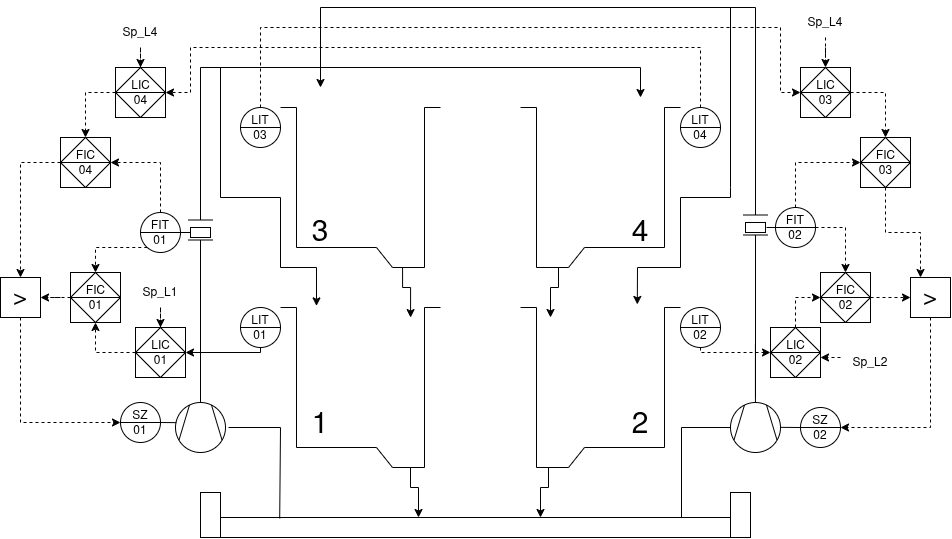
\includegraphics[width=0.95\textwidth]{img/planta_4_estanques_P&ID.png}
  \end{center}
  \caption{P\&ID de la planta de 4 estanques}\label{fig:p&id}
\end{figure}

\clearpage

\subsection{Parámetros del Sistema}

Para el desarrollo del modelo fenomenológico y las posteriores estrategias de control, se definen los parámetros físicos de la planta de 4 estanques. Los valores presentados en la Tabla \ref{tab:parametros} corresponden a las dimensiones físicas de los depósitos, las características de los actuadores y las constantes operativas del controlador ControlLogix.

Es imperativo destacar que el correcto levantamiento de estos parámetros es fundamental, ya que el algoritmo de prealimentación (Feed-Forward) invierte el modelo físico basándose estrictamente en estas magnitudes.

\begin{table}[ht]
    \centering
    \caption{Parámetros físicos y operativos de la Planta de 4 Estanques}
    \label{tab:parametros}
    \renewcommand{\arraystretch}{1.2} % Mejora el espaciado de las filas
    \begin{tabular}{llcc}
        \hline
        \textbf{Símbolo} & \textbf{Descripción} & \textbf{Valor} & \textbf{Unidad} \\
        \hline
        $A_1, A_3$ & Área transversal de los estanques impares & 0.159 & $m^2$ \\
        $A_2, A_4$ & Área transversal de los estanques pares & 0.159 & $m^2$ \\
        $a_1$ & Área del orificio de descarga (estanque 1) &  6.1360e-4 & $m^2$ \\
        $a_2$ & Área del orificio de descarga (estanque 2) & 5.4678e-4  & $m^2$ \\
        $a_3$ & Área del orificio de descarga (estanque 3) &  3.5752e-4 & $m^2$ \\
        $a_4$ & Área del orificio de descarga (estanque 4) &  4.1820e-4 & $m^2$ \\
        $k_1$ & Ganancia de la Bomba 1 (Variador 1) & 0.0017 & $(m^3/s)$ \\
        $k_2$ & Ganancia de la Bomba 2 (Variador 2) & 0.0017 & $(m^3/s)$ \\
        $\gamma_1$ & Fracción de flujo de la válvula de 3 vías (Bomba 1) & 0.455 & Adimensional \\
        $\gamma_2$ & Fracción de flujo de la válvula de 3 vías (Bomba 2) & 0.415 & Adimensional \\
        $g$ & Aceleración de la gravedad & 9.81 & $m/s^2$ \\
        $T_s$ & Tiempo de muestreo & 0.1 & $s$ \\
        \hline
    \end{tabular}
\end{table}

\clearpage
\subsection{Balance de Masas} % Ecuaciones diferenciales

El modelo fenomenológico de la planta se obtiene aplicando el principio de conservación de masa para cada depósito. La variación de volumen en el tiempo ($\frac{dV}{dt} = A \frac{dh}{dt}$) es igual a la suma de los caudales que ingresan menos los caudales que salen. 

Utilizando la Ley de Torricelli para modelar la descarga por gravedad a través de los orificios, la dinámica no lineal del sistema de cuatro estanques queda descrita por el siguiente conjunto de Ecuaciones Diferenciales Ordinarias (EDO):

\begin{align}
    A_1 \frac{dh_1}{dt} &= -a_1 \sqrt{2g h_1} + a_3 \sqrt{2g h_3} + \gamma_1 k_1 f_1 \label{eq:edo_h1} \\
    A_2 \frac{dh_2}{dt} &= -a_2 \sqrt{2g h_2} + a_4 \sqrt{2g h_4} + \gamma_2 k_2 f_2 \label{eq:edo_h2} \\
    A_3 \frac{dh_3}{dt} &= -a_3 \sqrt{2g h_3} + (1-\gamma_2) k_2 f_2 \label{eq:edo_h3} \\
    A_4 \frac{dh_4}{dt} &= -a_4 \sqrt{2g h_4} + (1-\gamma_1) k_1 f_1 \label{eq:edo_h4}
\end{align}

Donde la variable $h_i$ representa el nivel del estanque $i$, y $f_j$ corresponde a la señal de control aplicada a la bomba $j$. Los términos proporcionales a $\gamma$ y $(1-\gamma)$ reflejan la división del caudal en las válvulas.

\subsection{Discretización} % Euler

Para implementar las estrategias de control y realizar simulaciones computacionales, es necesario transformar el modelo continuo a su equivalente en tiempo discreto. Dado que los tiempos de muestreo ($T_s$) típicamente utilizados en la automatización de procesos industriales son pequeños en comparación con la constante de tiempo dominante de los estanques, el método de integración de Euler hacia adelante resulta suficiente y computacionalmente eficiente para el autómata.

Aproximando la derivada del nivel como la tasa de cambio entre dos instantes de muestreo consecutivos:
\begin{equation}
    \frac{dh(t)}{dt} \approx \frac{h[k+1] - h[k]}{T_s}
\end{equation}

Reemplazando esta aproximación en el balance de masas, se obtiene el sistema de ecuaciones en diferencias que predice el nivel en el instante futuro $[k+1]$ basándose en el estado actual $[k]$ y la acción de control actual $u[k]$:

\begin{align}
    h_1[k+1] &= h_1[k] + \frac{T_s}{A_1} \left( -a_1 \sqrt{2g h_1[k]} + a_3 \sqrt{2g h_3[k]} + \gamma_1 k_1 u_1[k] \right) \label{eq:disc_h1} \\
    h_2[k+1] &= h_2[k] + \frac{T_s}{A_2} \left( -a_2 \sqrt{2g h_2[k]} + a_4 \sqrt{2g h_4[k]} + \gamma_2 k_2 u_2[k] \right) \label{eq:disc_h2} \\
    h_3[k+1] &= h_3[k] + \frac{T_s}{A_3} \left( -a_3 \sqrt{2g h_3[k]} + (1-\gamma_2) k_2 u_2[k] \right) \label{eq:disc_h3} \\
    h_4[k+1] &= h_4[k] + \frac{T_s}{A_4} \left( -a_4 \sqrt{2g h_4[k]} + (1-\gamma_1) k_1 u_1[k] \right) \label{eq:disc_h4}
\end{align}

Estas ecuaciones discretas son la base tanto para la simulación de la planta en software externo como para la posterior deducción de los algoritmos de control digital implementados en el PLC.

\subsection{Modelo del Sistema}
\subsubsection{Linealización}
Tomando las ecuaciones \ref{eq:edo_h1}, \ref{eq:edo_h2}, \ref{eq:edo_h3} y \ref{eq:edo_h4}. Se aplica una aproximación de \textbf{Taylor} de primer orden, alrededor de los niveles en estado estacionario $(h_i^0, Q_{in}^0)$, definimos la función de descarga:

\begin{equation}
f(h_i) = a_i \sqrt{2g h_i} = a_i \sqrt{2g} \cdot h_i^{1/2}
\label{eq:func_descarga}
\end{equation}

Se aplica la expansión en Series de Taylor truncada al primer orden alrededor de $h_i^0$:

\begin{equation}
f(h_i) \approx f(h_i^0) + \left. \frac{df(h_i)}{dh_i} \right|_{h_i = h_i^0} (h_i - h_i^0)
\label{eq:taylor_exp}
\end{equation}

Se calcula la primera derivada de la función con respecto a $h_i$:

\begin{equation}
\frac{df(h_i)}{dh_i} = a_i \sqrt{2g} \left( \frac{1}{2} h_i^{-1/2} \right) = \frac{a_i \sqrt{2g}}{2\sqrt{h_i}}
\label{eq:derivada_f}
\end{equation}

Evaluando la derivada estrictamente en el punto de operación $h_i^0$ y reescribiendo algebraicamente para agrupar términos en la raíz:

\begin{equation}
\left. \frac{df(h_i)}{dh_i} \right|_{h_i = h_i^0} = \frac{a_i \sqrt{2g}}{\sqrt{4 h_i^0}} = a_i \sqrt{\frac{2g}{4 h_i^0}} = a_i \sqrt{\frac{g}{2 h_i^0}}
\label{eq:derivada_eval}
\end{equation}

Sustituyendo \eqref{eq:derivada_eval} en \eqref{eq:taylor_exp}, la aproximación lineal del flujo de salida es:

\begin{equation}
Q_{out} \approx a_i \sqrt{2g h_i^0} + \left( a_i \sqrt{\frac{g}{2 h_i^0}} \right) (h_i - h_i^0)
\label{eq:qout_aprox}
\end{equation}

\subsection{Variables de Desviación y Modelo LTI}
Se definen las variables de desviación respecto al punto de equilibrio:
\begin{align*}
\Delta h_i(t) &= h_i(t) - h_i^0 \\
\Delta Q_{in}(t) &= Q_{in}(t) - Q_{in}^0
\end{align*}

Reemplazando la aproximación \eqref{eq:qout_aprox} y las variables de desviación en la ecuación diferencial original, y sabiendo que en estado estacionario $Q_{in}^0 = a_i \sqrt{2g h_i^0}$ (por lo que se anulan), se obtiene:

\begin{equation}
A_i \frac{d(\Delta h_i(t))}{dt} = \Delta Q_{in}(t) - \left( a_i \sqrt{\frac{g}{2 h_i^0}} \right) \Delta h_i(t)
\label{eq:edo_desviacion}
\end{equation}

Dividiendo la expresión por el área del estanque $A_i$ para normalizar la derivada:

\begin{equation}
\frac{d(\Delta h_i(t))}{dt} = - \left( \frac{a_i}{A_i} \sqrt{\frac{g}{2 h_i^0}} \right) \Delta h_i(t) + \frac{1}{A_i} \Delta Q_{in}(t)
\label{eq:edo_normalizada}
\end{equation}

\subsection{Definición de la Constante de Tiempo ($T_i$)}
La ecuación \eqref{eq:edo_normalizada} corresponde a la forma canónica de un sistema lineal de primer orden LTI (Linear Time-Invariant):

\begin{equation}
\frac{dx(t)}{dt} = -\frac{1}{T} x(t) + K u(t)
\label{eq:lti_canonica}
\end{equation}

Por inspección directa entre las ecuaciones \eqref{eq:edo_normalizada} y \eqref{eq:lti_canonica}, se puede notar que el término recíproco de la constante de tiempo $T_i$ es:

\begin{equation}
\frac{1}{T_i} = \frac{a_i}{A_i} \sqrt{\frac{g}{2 h_i^0}}
\label{eq:ti_inversa}
\end{equation}

Despejando $T_i$, aparece la expresión final documentada en el modelo de Johansson \cite{johansson2000}:

\begin{equation}
T_i = \frac{A_i}{a_i} \sqrt{\frac{2 h_i^0}{g}}
\label{eq:ti_final}
\end{equation}

Esta deducción demuestra analíticamente que la inercia dinámica del sistema ($T_i$) no es constante, sino que depende de manera no lineal del nivel del líquido en el punto de operación $h_i^0$.

\subsection{Matriz de Transferencia y Análisis de Ceros de Transmisión}

Una vez obtenidas las constantes de tiempo ($T_i$) mediante la linealización de la Ley de Torricelli por Series de Taylor, es posible representar la dinámica completa de la Planta de Cuatro Estanques de Johansson en el dominio de la frecuencia. Este análisis revelará la influencia estructural de las válvulas de tres vías ($\gamma_1, \gamma_2$) sobre la naturaleza de la fase del sistema multivariable.

\subsubsection{Representación en el Dominio de Laplace}
Considerando que la planta física está construida con cilindros de dimensiones idénticas, se asume un área transversal uniforme tal que $A_1 = A_2 = A_3 = A_4 = A$. Bajo esta premisa, las razones de área se anulan ($\frac{A_i}{A_j} = 1$), simplificando el sistema de ecuaciones diferenciales a:

\begin{align}
\frac{dx_1}{dt} &= -\frac{1}{T_1} x_1 + \frac{1}{T_3} x_3 + \frac{\gamma_1 k_1}{A} u_1 \label{eq:dx1_dt_simp} \\
\frac{dx_2}{dt} &= -\frac{1}{T_2} x_2 + \frac{1}{T_4} x_4 + \frac{\gamma_2 k_2}{A} u_2 \label{eq:dx2_dt_simp} \\
\frac{dx_3}{dt} &= -\frac{1}{T_3} x_3 + \frac{(1-\gamma_2) k_2}{A} u_2 \label{eq:dx3_dt_simp} \\
\frac{dx_4}{dt} &= -\frac{1}{T_4} x_4 + \frac{(1-\gamma_1) k_1}{A} u_1 \label{eq:dx4_dt_simp}
\end{align}

Aplicando la Transformada de Laplace bajo condiciones iniciales nulas, y resolviendo para los estanques superiores (3 y 4), se obtiene:

\begin{align}
X_3(s) &= \frac{(1-\gamma_2) k_2 T_3 / A}{1 + sT_3} U_2(s) \label{eq:X3_s} \\
X_4(s) &= \frac{(1-\gamma_1) k_1 T_4 / A}{1 + sT_4} U_1(s) \label{eq:X4_s}
\end{align}

Sustituyendo \eqref{eq:X3_s} en la ecuación transformada del Estanque 1, y \eqref{eq:X4_s} en la del Estanque 2, se derivan las ecuaciones de los estanques maestros:

\begin{align}
X_1(s) &= \left( \frac{c_1 \gamma_1}{1 + sT_1} \right) U_1(s) + \left( \frac{c_1 (1-\gamma_2)}{(1+sT_1)(1+sT_3)} \right) U_2(s) \label{eq:X1_s} \\
X_2(s) &= \left( \frac{c_2 (1-\gamma_1)}{(1+sT_2)(1+sT_4)} \right) U_1(s) + \left( \frac{c_2 \gamma_2}{1 + sT_2} \right) U_2(s) \label{eq:X2_s}
\end{align}

Donde $c_1 = \frac{T_1 k_1}{A}$ y $c_2 = \frac{T_2 k_2}{A}$.

\subsubsection{Matriz de Transferencia $G(s)$}
El sistema MIMO (Múltiples Entradas, Múltiples Salidas) se define matricialmente como $X(s) = G(s)U(s)$:

\begin{equation}
G(s) = \begin{bmatrix} 
\frac{c_1 \gamma_1}{1 + sT_1} & \frac{c_1 (1-\gamma_2)}{(1+sT_1)(1+sT_3)} \\ 
\frac{c_2 (1-\gamma_1)}{(1+sT_2)(1+sT_4)} & \frac{c_2 \gamma_2}{1 + sT_2} 
\end{bmatrix}
\label{eq:matriz_Gs}
\end{equation}

Se observa que la diagonal principal rige la dinámica directa (primer orden), mientras que la anti-diagonal gobierna el acoplamiento cruzado (segundo orden).

\subsubsection{Cálculo de los Ceros de Transmisión Multivariables}
En un sistema MIMO cuadrado ($2 \times 2$), los ceros de transmisión corresponden a las raíces del polinomio resultante de igualar el determinante de la matriz de transferencia a cero:

\begin{equation}
\det(G(s)) = G_{11}G_{22} - G_{12}G_{21} = 0
\label{eq:det_Gs}
\end{equation}

Sustituyendo los elementos de la matriz y factorizando el término común $\frac{c_1 c_2}{(1+sT_1)(1+sT_2)}$:

\begin{equation}
\frac{c_1 c_2}{(1+sT_1)(1+sT_2)} \left[ \gamma_1 \gamma_2 - \frac{(1-\gamma_1)(1-\gamma_2)}{(1+sT_3)(1+sT_4)} \right] = 0
\label{eq:ceros_factorizado}
\end{equation}

Para encontrar los ceros, igualamos el término entre corchetes a cero y se multiplica por el denominador $(1+sT_3)(1+sT_4)$:

\begin{equation}
\gamma_1 \gamma_2 (1+sT_3)(1+sT_4) - (1-\gamma_1)(1-\gamma_2) = 0
\label{eq:ecuacion_ceros}
\end{equation}

Expandiendo el producto de las constantes de tiempo y agrupando los coeficientes según el grado de $s$:

\begin{equation}
s^2 [\gamma_1 \gamma_2 T_3 T_4] + s [\gamma_1 \gamma_2 (T_3+T_4)] + (\gamma_1 + \gamma_2 - 1) = 0
\label{eq:polinomio_caracteristico_ceros}
\end{equation}
\clearpage
\subsubsection{Análisis de Estabilidad y Fase del Sistema}
La Ecuación \eqref{eq:polinomio_caracteristico_ceros} es una cuadrática característica de los ceros del sistema. De acuerdo con el criterio de Routh-Hurwitz, para que las raíces se encuentren estrictamente en el Semiplano Izquierdo ($LHP$) de Laplace, todos los coeficientes del polinomio deben poseer el mismo signo positivo.

Dado que $T_3, T_4 > 0$ y $\gamma_1, \gamma_2 \in (0, 1)$, los coeficientes de $s^2$ y $s$ son constitutivamente positivos. Por lo tanto, la ubicación de los ceros depende exclusivamente del término independiente:

\textbf{Condición de Fase Mínima (Ceros LHP):}
Para un comportamiento controlable sin respuesta inversa transitoria, se requiere:
\begin{equation}
\gamma_1 + \gamma_2 - 1 > 0 \implies \gamma_1 + \gamma_2 > 1
\label{eq:condicion_fase_minima}
\end{equation}
Físicamente, esto indica que los flujos directos hacia los estanques inferiores dominan sobre el acoplamiento cruzado hacia los estanques superiores.

\textbf{Condición de Fase No Mínima (Ceros RHP):}
Bajo la configuración asignada al proyecto ($\gamma_1 = 0.455$, $\gamma_2 = 0.4195$), la suma resulta en $0.8745$.
\begin{equation}
\gamma_1 + \gamma_2 - 1 < 0 \implies \gamma_1 + \gamma_2 < 1
\label{eq:condicion_fase_no_minima}
\end{equation}
Esta inecuación \eqref{eq:condicion_fase_no_minima} demuestra que el término independiente es negativo. Según Routh-Hurwitz, la alternancia de signos en el polinomio garantiza la existencia de al menos una raíz en el Semiplano Derecho ($RHP$). Este Cero de Transmisión de Semiplano Derecho provoca matemáticamente el fenómeno de subamortiguación inicial (Undershoot) o Respuesta Inversa, limitando severamente la aplicabilidad de controladores PID de alta ganancia.
\clearpage
\subsection{Cálculo del Punto de Operación y Restricciones Estáticas}

Para determinar la viabilidad de un punto de operación $(h_1^0, h_2^0)$ y calcular los esfuerzos de control requeridos $(u_1^0, u_2^0)$, se debe analizar el sistema en estado estacionario. 

\subsubsection{Balance de Masa en Estado Estacionario}
Con base en las ecuaciones diferenciales no lineales del sistema, en estado estacionario o de equilibrio, no hay acumulación de volumen en los estanques, por lo que las derivadas del nivel con respecto al tiempo se igualan a cero ($\frac{dh_i}{dt} = 0$). 

Esto implica que el flujo volumétrico total que entra a cada estanque es exactamente igual al flujo que sale por gravedad (Ley de Torricelli):

\begin{align}
\text{Estanque 1:} \quad a_1 \sqrt{2g h_1^0} &= \gamma_1 k_1 u_1^0 + a_3 \sqrt{2g h_3^0} \label{eq:estatico_1} \\
\text{Estanque 2:} \quad a_2 \sqrt{2g h_2^0} &= \gamma_2 k_2 u_2^0 + a_4 \sqrt{2g h_4^0} \label{eq:estatico_2} \\
\text{Estanque 3:} \quad a_3 \sqrt{2g h_3^0} &= (1-\gamma_2) k_2 u_2^0 \label{eq:estatico_3} \\
\text{Estanque 4:} \quad a_4 \sqrt{2g h_4^0} &= (1-\gamma_1) k_1 u_1^0 \label{eq:estatico_4}
\end{align}

\subsubsection{Reducción del Sistema por Sustitución}
El objetivo es encontrar una relación directa entre los actuadores ($u_1, u_2$) y los niveles de los estanques maestros inferiores ($h_1, h_2$). 

Observando las ecuaciones \eqref{eq:estatico_3} y \eqref{eq:estatico_4}, notamos que los términos de descarga de los estanques superiores ($a_3 \sqrt{2g h_3^0}$ y $a_4 \sqrt{2g h_4^0}$) dependen de manera directa y lineal de los comandos de las bombas cruzadas.

Sustituyendo la ecuación \eqref{eq:estatico_3} en la ecuación \eqref{eq:estatico_1}:
\begin{equation}
a_1 \sqrt{2g h_1^0} = \gamma_1 k_1 u_1^0 + (1-\gamma_2) k_2 u_2^0
\label{eq:reducida_1}
\end{equation}

Sustituyendo la ecuación \eqref{eq:estatico_4} en la ecuación \eqref{eq:estatico_2}:
\begin{equation}
a_2 \sqrt{2g h_2^0} = (1-\gamma_1) k_1 u_1^0 + \gamma_2 k_2 u_2^0
\label{eq:reducida_2}
\end{equation}

\subsubsection{Representación Matricial (Matriz Estática)}
Para simplificar la notación, definimos los "Flujos de Fuga Deseados" en los estanques inferiores como constantes dependientes de los Setpoints:
\begin{align*}
F_1 &= a_1 \sqrt{2g h_1^0} \\
F_2 &= a_2 \sqrt{2g h_2^0}
\end{align*}

Reescribiendo las ecuaciones \eqref{eq:reducida_1} y \eqref{eq:reducida_2} en forma matricial, se obtiene la relación lineal que mapea los esfuerzos de control con los flujos de descarga en estado estacionario:

\begin{equation}
\begin{bmatrix} F_1 \\ F_2 \end{bmatrix} = 
\underbrace{
\begin{bmatrix} 
\gamma_1 k_1 & (1-\gamma_2) k_2 \\ 
(1-\gamma_1) k_1 & \gamma_2 k_2 
\end{bmatrix}
}_{M}
\begin{bmatrix} u_1^0 \\ u_2^0 \end{bmatrix}
\label{eq:matriz_estatica}
\end{equation}

Donde $M$ es la Matriz de Ganancia Estática del sistema.

\subsubsection{Cálculo de Actuadores y Restricciones}
Para encontrar los valores requeridos en las bombas para alcanzar un par de niveles $(h_1^0, h_2^0)$, se multiplica por la matriz inversa $M^{-1}$:

\begin{equation}
\begin{bmatrix} u_1^0 \\ u_2^0 \end{bmatrix} = M^{-1} \begin{bmatrix} F_1 \\ F_2 \end{bmatrix}
\label{eq:calculo_bombas}
\end{equation}

Dado que los actuadores tienen restricciones físicas irreducibles ($0 \le u_i \le 1.0$), cualquier vector de flujos $\begin{bmatrix} F_1 & F_2 \end{bmatrix}^T$ que requiera valores de $u$ fuera de este rango se considera un punto de operación físicamente inalcanzable.


\subsubsection{Ecuaciones Base según la Topología}
Siguiendo la arquitectura física de la planta, se establece el origen del agua para cada estanque en estado estacionario:

\begin{align}
F_4 &= (1-\gamma_1) k_1 u_1 \quad \text{(El estanque 4 solo depende de la Bomba 1)} \label{eq:F4_u1} \\
F_3 &= (1-\gamma_2) k_2 u_2 \quad \text{(El estanque 3 solo depende de la Bomba 2)} \label{eq:F3_u2} \\
F_1 &= \gamma_1 k_1 u_1 + F_3 \quad \text{(El estanque 1 recibe de la Bomba 1 y del Estanque 3)} \label{eq:F1_dependencia} \\
F_2 &= \gamma_2 k_2 u_2 + F_4 \quad \text{(El estanque 2 recibe de la Bomba 2 y del Estanque 4)} \label{eq:F2_dependencia}
\end{align}

\subsubsection{El Compromiso del Actuador 1}
Al defininir un \textit{Setpoint} fijo para el Estanque 1, $F_1$ se convierte en una constante conocida. 

Sustituyendo \eqref{eq:F3_u2} en \eqref{eq:F1_dependencia}, Se obtiene la ecuación fundamental que vincula a ambas bombas para satisfacer al Estanque 1:
\begin{equation}
F_1 = \gamma_1 k_1 u_1 + (1-\gamma_2) k_2 u_2
\label{eq:vinculo_bombas}
\end{equation}

Despejando el esfuerzo de la Bomba 1 ($u_1$) necesario para mantener este nivel:
\begin{equation}
u_1 = \frac{F_1 - (1-\gamma_2) k_2 u_2}{\gamma_1 k_1}
\label{eq:u1_despejado}
\end{equation}

\textit{Físicamente, esta ecuación demuestra que si la Bomba 2 ($u_2$) inyecta mucha agua al Estanque 3 (que luego cae al Estanque 1), la Bomba 1 ($u_1$) se ve obligada a reducir su esfuerzo para no sobrepasar el Setpoint $F_1$.}

\subsubsection{Los Límites Físicos}
Las bombas tienen límites físicos absolutos: no pueden operar a potencia negativa ni superar el 100\% de su capacidad. Por lo tanto:
\begin{equation*}
0 \le u_1 \le 1.0 \quad \text{(asumiendo $u_1$ normalizado entre 0 y 1)}
\end{equation*}

Aplicando este límite físico a nuestra ecuación \eqref{eq:u1_despejado}:
\begin{equation}
0 \le \frac{F_1 - (1-\gamma_2) k_2 u_2}{\gamma_1 k_1} \le 1.0
\end{equation}

Al despejar $u_2$ de esta inecuación doble, es evidente que la simple exigencia de mantener el Estanque 1 obliga a la Bomba 2 a operar dentro de un rango cerrado:

\textbf{Límite por apagado de Bomba 1 ($u_1 \ge 0$):}
\begin{equation}
u_2 \le \frac{F_1}{(1-\gamma_2)k_2}
\label{eq:u2_maximo}
\end{equation}

\textbf{Límite por saturación de Bomba 1 ($u_1 \le 1.0$):}
\begin{equation}
u_2 \ge \frac{F_1 - \gamma_1 k_1}{(1-\gamma_2)k_2}
\label{eq:u2_minimo}
\end{equation}

\textit{Conclusión intermedia: Al fijar $h_1$, la Bomba 2 pierde su libertad total de [0 a 100\%] y queda atrapada entre estos dos valores.}

\subsubsection{Repercusión en el Estanque 2 (El Rango Válido)}
Finalmente, tomando la ecuación base \eqref{eq:F2_dependencia} y Sustituyendo $F_4$ usando \eqref{eq:F4_u1}:
\begin{equation}
F_2 = \gamma_2 k_2 u_2 + (1-\gamma_1) k_1 u_1
\end{equation}

Para ver la dependencia total, se sustituye $u_1$ usando la ecuación \eqref{eq:u1_despejado}:
\begin{equation}
F_2 = \gamma_2 k_2 u_2 + (1-\gamma_1) k_1 \left[ \frac{F_1 - (1-\gamma_2) k_2 u_2}{\gamma_1 k_1} \right]
\end{equation}

Simplificando los términos $k_1$ y agrupando lo que multiplica a $F_1$ y lo que multiplica a $u_2$:
\begin{equation}
F_2 = \left( \frac{1-\gamma_1}{\gamma_1} \right) F_1 + \left[ \frac{\gamma_1 \gamma_2 - (1-\gamma_1)(1-\gamma_2)}{\gamma_1} \right] k_2 u_2
\end{equation}

Reduciendo el término entre corchetes, se llega a la ecuación maestra de la planta:
\begin{equation}
F_2 = \underbrace{\left( \frac{1-\gamma_1}{\gamma_1} \right) F_1}_{\text{Constante impuesta por } h_1} + \underbrace{\left( \frac{\gamma_1 + \gamma_2 - 1}{\gamma_1} \right)}_{\text{Pendiente negativa}} k_2 u_2
\label{eq:F2_final}
\end{equation}
\clearpage

\section{Diseño del Sistema de Control}

    \subsection{Control en Cascada} % LIC -> FIC

La arquitectura de control base seleccionada para cada línea de los depósitos corresponde a un esquema en Cascada. Esta topología se justifica teóricamente por la existencia de dos dinámicas temporales claramente separadas: la dinámica rápida del actuador y la tubería (flujo), y la dinámica lenta de acumulación de masa (nivel del estanque).

El esquema se compone de dos lazos anidados:
\begin{itemize}
    \item \textbf{Lazo Interno (Esclavo - FIC):} Su objetivo es controlar el caudal inyectado al sistema. Posee una dinámica rápida y su función principal es rechazar las perturbaciones locales del actuador (como variaciones en la presión de la línea, desgaste mecánico de la bomba o histéresis) antes de que afecten a la variable principal. Al sintonizar este lazo, el conjunto actuador-tubería se linealiza desde la perspectiva del controlador maestro.
    \item \textbf{Lazo Externo (Maestro - LIC):} Su objetivo es controlar el nivel del estanque ($h_i$). Su salida de control no ataca directamente al variador de frecuencia, sino que establece el *Setpoint* dinámico ($SP_{flujo}$) que el lazo esclavo debe seguir.
\end{itemize}

Matemáticamente, la señal de control final $u(t)$ enviada al variador de frecuencia es calculada por el algoritmo discreto del FIC, cuyo error se define como $e_{flujo}[k] = LIC_{out}[k] - FIT[k]$. Esta separación de dinámicas permite utilizar sintonías más agresivas en el control de nivel sin comprometer la estabilidad ante imperfecciones mecánicas.
    \subsection{Lógica de Selección (Override)} % Bloques TY
    Como el sistema es sub-actuado ya que cuenta con 4 salidas pero sólo 2 actuadores, no es posible controlar los estanque $1$ y $4$ o $2$ y $3$.

    Es por esto que se implementa un algoritmo de selección entre las señales al actuador, esto se desglosa en la siguiente tabla:

    $$\begin{bmatrix}
    >: \text{Flujo mayor}\\
    <: \text{Flujo menor}\\
  e: \text{Mayor error}
    \end{bmatrix}$$
\clearpage
    \subsection{Feed-Forward (Prealimentación)} % G_h y G_w


El control retroalimentado (Feedback) tradicional posee una limitación inherente: requiere que exista un error en la variable de proceso para poder actuar. Para compensar esta inercia, se implementa una arquitectura de prealimentación o \textit{Feedforward} (FF), la cual mide las variables de entrada al sistema e inyecta una acción de control antes de que la variable controlada se vea afectada.

\begin{figure}[ht]
  \begin{center}
    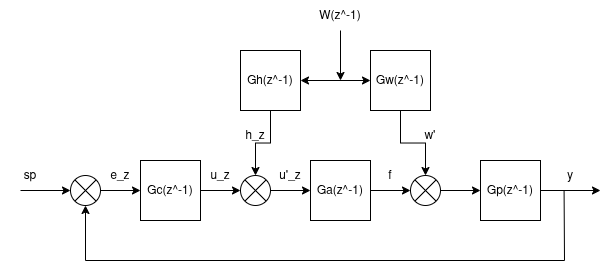
\includegraphics[width=0.95\textwidth]{img/ff.png}
  \end{center}
  \caption{}\label{fig:ff}
\end{figure}
\subsubsection{Obtención Matemática: Compensación de Perturbaciones}

Considérese un sistema donde la salida $y(z^{-1})$ se ve afectada tanto por la acción de control $u_z$ a través de la planta $G_p(z^{-1})$ y el actuador $G_a(z^{-1})$, como por una perturbación medible $W(z^{-1})$ a través de su propia dinámica $G_w(z^{-1})$. La ecuación en el dominio $Z$ es:
\[
  Y(z^{-1}) =G_p(z^{-1}) \left[ (u_{z}(z^{-1}) + h_{h}(z^{-1})) G_a(z^{-1}) + W(z^{-1}) G_w(z^{-1}) \right]
\]
\[
Y(z^{-1}) = G_p(z^{-1})\left[ (u_{z}(z^{-1}) + W(z^{-1})G_h(z^{-1})) G_a(z^{-1})  + W(z^{-1}) G_w(z^{-1})\right]
\]
\[ 
  Y(z^{-1}) = G_p(z^{-1})\left[u_z(z^{-1})G_a(z^{-1})G_p(z^{-1}) + W(z^{-1})G_h(z^{-1})G_a(z^{-1}) + W(z^{-1})G_w(z^{-1})\right]  
\]

\begin{equation}
  Y(z^{-1}) = \underbrace{(Sp - Pv)G_c(z^{-1})G_a(z^{-1})G_p(z^{-1})}_{\text{PID}} + \underbrace{W(z^{-1})G_h(z^{-1})G_a(z^{-1})G_p(z^{-1}) + W(z^{-1})G_w(z^{-1})G_p(z^{-1})}_{\text{Feed-Forward}}  
  \label{eq:ff2}
\end{equation}

\clearpage


El objetivo del compensador de perturbaciones es lograr una invariancia perfecta, es decir, que el efecto de $W(z^{-1})$ sobre $Y(z^{-1})$ sea nulo ($Y(z^{-1}) = 0$ asumiendo $u_{z}=0$). Igualando a cero la contribución de la perturbación, se despeja la acción de control anticipatoria:
\[
  0 = W(z^{-1})G_h(z^{-1})G_a(z^{-1})G_p(z^{-1}) + W(z^{-1})G_w(z^{-1})G_p(z^{-1}) 
\]

\begin{equation}
  G_h(z^{-1}) = -\frac{G_w(z^{-1})}{G_a(z^{-1})} 
  \label{eq:G_w}
\end{equation}
Definiendo el bloque compensador como $
  G_h(z^{-1}) = -\frac{G_w(z^{-1})}{G_a(z^{-1})} 
$, se logra la cancelación algebraica de la perturbación entrante.

\subsubsection{Obtención Matemática: Seguimiento de Referencia (Setpoint)}
Se puede aplicar un raciocinio idéntico para mejorar el seguimiento de la referencia ($SP$). En lugar de esperar a que el integrador del PID acumule la energía necesaria para alcanzar el nivel deseado, se puede pre-calcular el esfuerzo de control exacto. 

Es fundamental destacar que \textbf{no se invierte la dinámica completa de la planta} (lo cual requeriría la derivada de la referencia y generaría un esfuerzo de control irrealizable). En su lugar, el Feedforward de Setpoint invierte únicamente la \textbf{ganancia estática} del proceso. 

En sistemas con dinámicas complejas como el de los 4 estanques, esta ganancia estática contiene la principal no linealidad del sistema (la fuga parabólica de Torricelli). Al inyectar una señal de prealimentación que es la inversa exacta de esta no linealidad ($G_{sp} = G_{estatico}^{-1}$), se logran dos objetivos simultáneos:

\begin{enumerate}
    \item Proporcionar al actuador la energía base requerida para sostener el nivel del Setpoint deseado en estado estacionario.
    \item Linealizar el sistema desde la perspectiva del lazo cerrado, permitiendo que el controlador PID solo deba encargarse de corregir las inercias transitorias dinámicas y los pequeños errores de modelación.
\end{enumerate}


\begin{figure}[ht]
  \begin{center}
    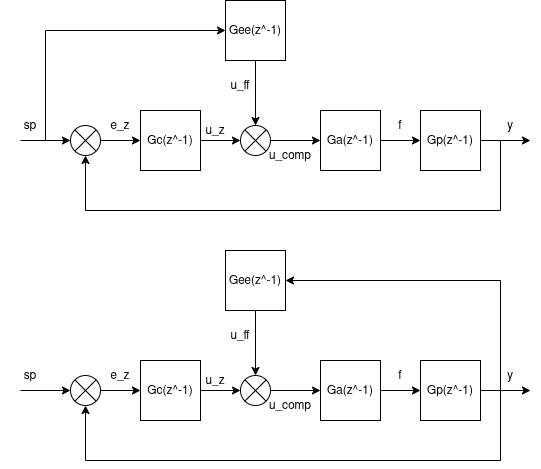
\includegraphics[width=0.8\textwidth]{img/ff_sp.png}
  \end{center}
  \caption{}\label{fig:ffsp}
\end{figure}

Ignorando la perturbación y la acción del controlador temporalmente, se busca que la salida alcance la referencia ($Y(z^{-1}) = SP(z^{-1})$) utilizando exclusivamente una acción precalculada $U_{FF\_SP}(z^{-1})$:

\begin{align}
    SP(z^{-1}) &= U_{FF\_SP}(z^{-1}) G_a(z^{-1}) G_p(z^{-1}) \\
    U_{FF\_SP}(z^{-1}) &= SP(z^{-1}) \frac{1}{G_a(z^{-1}) G_p(z^{-1})}
\end{align}

Definiendo este segundo bloque como $G_{sp}(z^{-1}) = \frac{1}{G_a(z^{-1}) G_p(z^{-1})}$, se establece un control de \textit{2 Grados de Libertad}, donde el Feedforward proporciona el esfuerzo base y el PID se encarga únicamente de corregir errores dinámicos y no linealidades residuales no modeladas.

\subsubsection{Aplicación a las Ecuaciones de Diferencias de la Planta}
Para aplicar esta teoría lineal a los estanques no lineales, evaluamos la derivada del balance de masas en estado estacionario ($\frac{dh}{dt} = 0$). Tomando como ejemplo el Estanque 1 (que sufre la perturbación de caudal del Estanque 3), la Ecuación \ref{eq:edo_h1} se iguala a cero.

Forzando que en estado estacionario el nivel alcance el Setpoint ($h_1 = SP_1$), y despejando la acción de control de la bomba ($u_1$), obtenemos la ley de control Feedforward pura (sin considerar aún la acción del PID):
\begin{align}
    0 &= -a_1 \sqrt{2g \cdot SP_1} + a_3 \sqrt{2g \cdot h_3} + \gamma_1 k_1 u_1 \nonumber \\
    \gamma_1 k_1 u_1 &= a_1 \sqrt{2g \cdot SP_1} - a_3 \sqrt{2g \cdot h_3} \nonumber \\
    u_1 &= \underbrace{\frac{a_1 \sqrt{2g \cdot SP_1}}{\gamma_1 k_1}}_{\text{Término } G_h \text{ (Referencia)}} - \underbrace{\frac{a_3 \sqrt{2g \cdot h_3}}{\gamma_1 k_1}}_{\text{Término } C_w \text{ (Perturbación)}}
\end{align}

Al integrar esto con el algoritmo digital dentro del PLC, la señal de control total en el instante discreto $[k]$ resulta en la suma de prealimentación y el control retroalimentado:
\begin{equation}
    u_{total}[k] = u_{PID}[k] + \frac{a_1 \sqrt{2g \cdot SP_1[k]}}{\gamma_1 k_1} - \frac{a_3 \sqrt{2g \cdot h_3[k]}}{\gamma_1 k_1}
\end{equation}

\clearpage
\subsection{Arquitecturas de Inyección del Feedforward en Cascada}

Al implementar la estrategia de prealimentación junto con un control en cascada (LIC $\rightarrow$ FIC) en Texto Estructurado, existen dos topologías matemáticas válidas para inyectar el Feedforward. La elección depende de si se prioriza la robustez del lazo o la velocidad de rechazo de la perturbación.

\subsubsection{Arquitectura 1: Inyección en el Setpoint del Lazo Esclavo}
En este enfoque, el Feedforward se suma a la salida del controlador maestro (LIC). Dado que el Setpoint del lazo de flujo (FIC) debe estar en unidades de caudal ($cm^3/s$ o $L/min$), la ecuación de prealimentación \textbf{no debe incluir la ganancia de la bomba ($k_1$)}. 

La secuencia de cálculo discreto en el instante $[k]$ es:
\begin{align}
    Q_{FF}[k] &= \frac{a_1 \sqrt{2g \cdot SP_1[k]}}{\gamma_1} - \frac{a_3 \sqrt{2g \cdot h_3[k]}}{\gamma_1} \label{eq:ff_caudal} \\
    SP_{FIC}[k] &= CV_{LIC}[k] + Q_{FF}[k] \label{eq:sp_fic_sum} \\
    u_1[k] &= CV_{FIC}[k] \label{eq:u_arch1}
\end{align}

\textbf{Ventaja:} Es la arquitectura más robusta. El FIC es el único encargado de gobernar la señal hacia el actuador ($u_1[k]$), por lo que su término integral mantiene el control total sobre la linealidad de la bomba sin sufrir problemas de \textit{windup} por señales externas.

\subsubsection{Arquitectura 2: Inyección a la Salida del Lazo Esclavo}
En este enfoque, el controlador de nivel (LIC) ataca directamente al Setpoint del flujo, y el Feedforward se inyecta en la etapa final, sumándose a la salida del FIC. En este caso, el Feedforward debe calcular \textbf{esfuerzo de control (Hz o Voltaje)}, por lo que la ganancia de la bomba ($k_1$) es indispensable en el denominador.

La secuencia de cálculo discreto en el instante $[k]$ es:
\begin{align}
    SP_{FIC}[k] &= CV_{LIC}[k] \label{eq:sp_fic_direct} \\
    u_{FF}[k] &= \frac{a_1 \sqrt{2g \cdot SP_1[k]}}{\gamma_1 k_1} - \frac{a_3 \sqrt{2g \cdot h_3[k]}}{\gamma_1 k_1} \label{eq:ff_esfuerzo} \\
    u_1[k] &= CV_{FIC}[k] + u_{FF}[k] \label{eq:u_arch2}
\end{align}

\textbf{Ventaja y Precaución:} Esta arquitectura garantiza un rechazo de perturbaciones casi instantáneo, ya que la señal de compensación ($u_{FF}[k]$) llega directamente al actuador saltándose la inercia dinámica del algoritmo del FIC. Sin embargo, al sumar una señal externa a la salida de un PID discreto implementado en Texto Estructurado, es estrictamente necesario aplicar técnicas de recálculo hacia atrás (\textit{back-calculation}) en el término integral del FIC; de lo contrario, el controlador asumirá que la perturbación fue un error propio e intentará cancelarla, desestabilizando el sistema.



\subsubsection{Solución Híbrida: Doble Inyección (Feedforward Coordinado)}

Si los requerimientos del proceso exigen la velocidad de reacción de la \textbf{Arquitectura 2} (inyección directa al actuador), pero se desea evitar el conflicto con la acción Proporcional e Integral del lazo esclavo en un entorno de Texto Estructurado puro, la solución matemática es implementar una \textit{Doble Inyección}.

Este método consiste en calcular simultáneamente el Feedforward en unidades de caudal ($Q_{FF}$) y en unidades de esfuerzo de control ($u_{FF}$), inyectándolos en ambos extremos del controlador esclavo (FIC) al mismo tiempo. De esta forma, se logra la corrección instantánea en la bomba, mientras se enmascara la perturbación modificando el Setpoint del FIC, lo que mantiene el error del esclavo cercano a cero y anula cualquier intento de contramedida.

La secuencia de cálculo discreto para la doble inyección en el instante $[k]$ es:

1. \textbf{Cálculo del requerimiento físico (Caudal):}
   $$Q_{FF}[k] = \frac{a_1 \sqrt{2g \cdot SP_1[k]}}{\gamma_1} - \frac{a_3 \sqrt{2g \cdot h_3[k]}}{\gamma_1}$$

 2. \textbf{Transformación a esfuerzo de control:}
   $$u_{FF}[k] = \frac{Q_{FF}[k]}{k_1}$$

 3. \textbf{Inyección 1: Ajuste del Setpoint (Pre-compensación):}
   $$SP_{FIC}[k] = CV_{LIC}[k] + Q_{FF}[k]$$

 4. \textbf{Cálculo del error y algoritmo del controlador (FIC):}
   $$e_{FIC}[k] = SP_{FIC}[k] - FIT_1[k]$$
   $$CV_{FIC}[k] = \text{PID}(e_{FIC}[k])$$

   5. \textbf{Inyección 2: Acción directa al actuador (Salida final):}
   $$u_1[k] = CV_{FIC}[k] + u_{FF}[k]$$

---

\textbf{Análisis de Dinámica:} Al momento de ocurrir la perturbación, $u_{FF}[k]$ altera el variador de frecuencia en el mismo ciclo de \textit{Scan}, garantizando un rechazo inmediato. Físicamente, el flujo $FIT_1$ cambia drásticamente. Sin embargo, como el término $Q_{FF}[k]$ fue sumado al $SP_{FIC}$, la ecuación del error ($e_{FIC}$) evalúa esta alza de flujo como el seguimiento exitoso de su nueva referencia. El lazo esclavo se mantiene estable y la cascada no se rompe..


\subsection{Selección de Arquitectura Feedforward en Cascada}

La elección entre inyectar la prealimentación en el Setpoint del esclavo (Arquitectura 1), en la salida del esclavo (Arquitectura 2) o utilizar una Doble Inyección (Arquitectura 3), no posee una respuesta única. El ingeniero de control debe evaluar los siguientes criterios de diseño:

\begin{enumerate}
    \item \textbf{Dinámica Relativa (Velocidad de Respuesta):}
    \begin{itemize}
        \item Si la dinámica del lazo esclavo (FIC) es al menos 5 a 10 veces más rápida que la perturbación, la \textbf{Arquitectura 1 (Setpoint)} es suficiente. El FIC reaccionará tan rápido al cambio de su referencia que el error temporal será despreciable.
        \item Si el actuador es lento o posee un tiempo muerto significativo, se prefiere la \textbf{Doble Inyección} para enviar el comando de voltaje inmediatamente y ganar tiempo físico, mientras se coordina con el PID.
    \end{itemize}

    \item \textbf{Nivel de Ruido en la Perturbación (Chattering):}
    \begin{itemize}
        \item El cálculo del Feedforward depende directamente de las mediciones de los sensores (en este caso, los transmisores de nivel $LIT$). Si esta señal es ruidosa (ej. oleaje en el estanque), la inyección directa a la salida transmitirá ese ruido amplificado directamente a la bomba, causando desgaste mecánico prematuro.
        \item En presencia de ruido, la \textbf{Arquitectura 1} es superior, ya que el algoritmo integral del FIC actúa como un filtro pasabajos (amortiguador) natural antes de que la señal llegue a la bomba.
    \end{itemize}

    \item \textbf{Herramientas de Programación (Bloques vs. ST puro):}
    \begin{itemize}
        \item Si el autómata dispone de bloques de control avanzados (como la instrucción \texttt{PIDE} en ControlLogix) que gestionan automáticamente el \textit{back-calculation} en su pin \texttt{FF}, la \textbf{Doble Inyección} se vuelve trivial de implementar y es altamente recomendada.
        \item Si el control debe ser programado desde cero mediante ecuaciones en diferencias en Texto Estructurado (ST), la \textbf{Arquitectura 1} es mandatoria para evitar un desarrollo de software excesivamente complejo y propenso a fallos matemáticos por \textit{Integral Windup}.
    \end{itemize}

    \item \textbf{Saturación y Seguridad del Actuador:}
    \begin{itemize}
        \item En la inyección a la salida, si el PID pide 40 Hz y el FF pide 20 Hz, la suma exige 60 Hz. Como el variador satura a 50 Hz, el sistema físico se limita, pero el PID interno no lo sabe y su integrador colapsa. Al inyectar en el Setpoint (Arquitectura 1), el FIC gestiona la saturación internamente y congela su integrador (\textit{Anti-Windup}) de forma natural.
    \end{itemize}
\end{enumerate}

\section{Implementación y Automatización}
\subsection{Instrumentación}
\subsubsection{Obtención Experimental de la Ganancia de la Bomba ($k_i$)}

En el desarrollo del modelo matemático, se asume que el caudal inyectado al sistema ($q_i$) es directamente proporcional a la señal de control enviada al variador de frecuencia ($u_i$). Esta relación se modela mediante la ganancia estática del actuador:
\begin{equation}
    q_i = k_i \cdot u_i
\end{equation}

Donde $k_i$ posee unidades de $\left[ \frac{\text{Caudal}}{\text{Esfuerzo}} \right]$ (por ejemplo, $\frac{L/min}{\text{Hz}}$ o $\frac{cm^3/s}{\%}$).

Para obtener este parámetro empíricamente en la planta física, se debe levantar una \textbf{curva de calibración de estado estacionario} operando el sistema en lazo abierto. El procedimiento estándar es el siguiente:

\begin{enumerate}
    \item \textbf{Modo Manual:} Se debe asegurar que el controlador de la bomba (FIC) se encuentre en modo manual, deshabilitando cualquier acción de control PID o Feedforward.
    \item \textbf{Inyección de Escalones:} Se aplican diferentes niveles de esfuerzo de control escalonados a la bomba, cubriendo su rango de operación normal (por ejemplo, $u = 20\%, 40\%, 60\%, 80\%$).
    \item \textbf{Registro de Estado Estacionario:} Para cada nivel de esfuerzo, se espera a que la dinámica de la tubería se estabilice y se registra el valor de caudal entregado por el transmisor de flujo (\textit{FIT}).
    \item \textbf{Regresión Lineal:} Se grafica el Caudal medido ($y$) versus el Esfuerzo de control ($x$). En la región lineal de operación de la bomba, los puntos formarán una recta. La constante $k_i$ corresponde a la pendiente de esta recta:
    \begin{equation}
        k_i = \frac{\Delta q}{\Delta u} = \frac{q_B - q_A}{u_B - u_A}
    \end{equation}
\end{enumerate}
    \subsection{Programación en Texto Estructurado}
    \subsection{Configuración de Red y Adquisición (OPC)}

\section{Diseño de la Interfaz Hombre-Máquina (HMI)}
La supervisión y operación de la planta se centralizó en una interfaz gráfica desarrollada en \textit{FactoryTalk View Studio}. Para asegurar una operación segura, eficiente y libre de fatiga visual, el desarrollo de las pantallas se rigió estrictamente por el estándar internacional de HMI de Alto Desempeño (High-Performance HMI) y la normativa interna del laboratorio.

\subsection{Filosofía de Diseño ISA-101}
El diseño visual se fundamenta en los lineamientos de la norma \textbf{ANSI/ISA-101.01}, cuyo objetivo principal es maximizar la \textit{Conciencia Situacional} (Situational Awareness) del operador y reducir su carga cognitiva. Para lograr esto en el proyecto, se implementaron las siguientes directrices:

\begin{itemize}
    \item \textbf{Paleta de Colores Atenuada:} Se eliminaron los fondos oscuros o de colores saturados típicos de interfaces antiguas. En su lugar, el sinóptico de la planta utiliza un fondo gris neutro (escala de grises). Los equipos dinámicos (estanques, tuberías, bombas) se dibujaron con bajo contraste durante su operación normal.
    \item \textbf{Uso Estratégico del Color:} Siguiendo la filosofía de "pantallas aburridas para procesos normales", colores llamativos como el rojo, amarillo o magenta fueron eliminados completamente de la paleta base y se reservaron \textbf{exclusivamente} para indicar condiciones anormales o estados de alarma. 
    \item \textbf{Jerarquía Visual e Interactividad:} Se estableció una distinción clara entre variables de solo lectura (valores de transmisores) y variables de escritura (Setpoints o salidas manuales). Los elementos interactivos, como los selectores de modo (Auto/Manual o Local/Remoto) para las bombas, utilizan un efecto de relieve (\textit{Raised}) para indicar que son botones accionables, previniendo errores de operación.
    \item \textbf{Navegación Eficiente:} Se implementó una estructura de pantallas por niveles (Nivel 1: Sinóptico general, Nivel 2: Tendencias detalladas y sintonización), accesible mediante un menú de navegación persistente con un máximo de 2 clics para alcanzar cualquier información crítica.
\end{itemize}

\subsection{Jerarquía de Alarmas y Eventos}
El sistema de alarmas no solo notifica fallas, sino que guía la respuesta del operador. La configuración en el servidor de \textit{FactoryTalk Alarms and Events} se estructuró separando claramente los \textbf{Eventos} (acciones normales de registro, como el cambio de un Setpoint o el inicio del \textit{Data Logging}) de las \textbf{Alarmas} (condiciones físicas anormales que requieren intervención inmediata).

Para las variables análogas críticas, particularmente el nivel de los 4 estanques ($LIT\_01$ a $LIT\_04$), se definió una matriz de alarmas basada en cuatro umbrales operativos, codificados visualmente según el estándar del proyecto:

\begin{table}[h]
\centering
\caption{Jerarquía y Codificación Visual de Alarmas (Estándar UdeC / ISA-101)}
\label{tab:alarmas}
\begin{tabular}{|l|c|l|l|}
\hline
\textbf{Estado} & \textbf{Límite} & \textbf{Prioridad} & \textbf{Color Asociado (HMI)} \\ \hline
Muy Alto & HH & Crítica & Rojo \\ \hline
Alto & H & Advertencia & Amarillo \\ \hline
Bajo & L & Advertencia & Amarillo \\ \hline
Muy Bajo & LL & Crítica & Rojo \\ \hline
\end{tabular}
\end{table}

\subsubsection{Estados de Reconocimiento}
Para cumplir con la gestión del ciclo de vida de la alarma, la HMI representa dinámicamente el estado de reconocimiento por parte del operador:
\begin{itemize}
    \item \textbf{Alarma Activa No Reconocida:} El indicador del estanque y el banner de alarmas destellan (\textit{Blinking}) en el color correspondiente (Rojo/Amarillo), exigiendo la atención del usuario.
    \item \textbf{Alarma Activa Reconocida (ACK):} Tras la confirmación del operador mediante el botón \textit{Acknowledge}, el destello cesa y el indicador se mantiene en color sólido mientras la condición de falla (ej. estanque rebalsando) persista físicamente en el PLC.
    \item \textbf{Retorno a la Normalidad (RTN):} Una vez que la variable física regresa a su rango operativo seguro, la alarma se despeja de la lista activa y queda registrada en el sumario histórico en color Azul.
\end{itemize}

\clearpage
\addcontentsline{toc}{section}{Bibliografía}
\renewcommand{\refname}{Bibliografía}
\nocite*{}
\bibliographystyle{ieeetr}
\bibliography{Referencias}

% \input{Contenidos/Z-Anexos}

\end{document}
